%%%%%%%%%%%%%%%%%%%%%%%%%%%%%%%%%%%%%%%%%%%%%%%%%%%%%%%
% LaTeX Template of MIST Thesis 
% Version 3.6 Date 27-03-2022
% Email: h.nyeem@eece.mist.ac.bd 
% -----------------------------------------------------
% This LaTeX template was originally developed by Lt Col Hussain Md Abu Nyeem, PhD, EME for the MSc Thesis students of the Military Institute of Science and Technology (MIST). The sucessive developments received updates with the specific policy and guidelines of MIST with a notable contribution of Major Md Abdul Wahed.
%
% This version quickly attempts for the first time to capture the prescribed format of the undergrad and postgrad theses of MIST students. This means that there would be surely some bugs and rooms for improvement.
%
% The main objective of this template is to fascilitate the existing BSc/MSc/PhD Students of MIST to easily typeset their thesis content. This means that once the input-data of the title page are given, most of the sections of the front- and back-matters will be generated automatically.
%
% Please send us the email for further development of this template

%------------------------------------------------------
%HOW TO USE (A Brief Guideline for the Beginner)
%------------------------------------------------------
%1. Input the data for the fornt matters starting lines from: 296 
%
%2. Images are to be copied in the FIGURE folder
%
%3. Update the Chapters in the CHAPTERS folder with the desired content
%
%4. Typesetting of abstract in Bengali is not yet supported by this version. However, a pre-typeset Bengali-abstract (written with avro in word or google doc, and saved as pdf) can be included in the abstract section.
%
%5. Update the ACKNOWLEDGEMENT, ABSTRACT, ABBREVIATIONS, SYMBOLS, ListOfPublication, and INDEX files in the CHAPTERS folder as well. Other pages of the front- and back-matters will be generated automatically.
%
%6. Reference files (bibtex files) are to be stored in the main dirctory where this file resides and the name of the bibtex file should be included in the \bibliography{FILENAME} in the REFERENCE section at the end of this document. Or, you may use/update the bibliographies in the current MyReference.bib file without further changes.


%%%%%%%%%%%%%%%%%%%%%%%%%%%%%%%%%%%%%%%%%%%%%%%%%%%%%%%
\pdfoptionpdfminorversion=5
%\RequirePackage{pdf14}
\documentclass[final,print]{packages/mistthesis} 
%%% REFFF
\usepackage[english]{babel}
\usepackage[labelformat=simple]{subcaption}    %%Adding option to remove parenthesis
\renewcommand{\thesubfigure}{\normalsize Figure \thefigure. (\alph{subfigure}):}
\usepackage[utf8x]{inputenc}
%%%%%%%%%%%%%%%%%%%%%%%%%% this makes the citation format correct
% \usepackage{natbib}
% \usepackage{fancyhd}
% \bibliographystyle{agsm}
\usepackage{apacite}
\AtBeginDocument{\renewcommand{\url}[1]{\relax}}
\pdfminorversion=6
\usepackage{times}
%\usepackage{mathpazo}
\usepackage{notoccite}
\usepackage{mfirstuc}
%include the preposition and conjunction used in your thesis title
\MFUnocap{the}\MFUnocap{and}\MFUnocap{in}\MFUnocap{on}
\MFUnocap{of}\MFUnocap{for}\MFUnocap{to}\MFUnocap{based}
\MFUnocap{a}\MFUnocap{an}
%\MFUnocap{to}\MFUnocap{based}

\usepackage{emptypage} 
%\renewcommand{\sfdefault}{\rmdefault}
%\usepackage{pdflscape}
\usepackage{rotating}
\usepackage{afterpage}
\newcommand\blankpage{
	\null
	\thispagestyle{empty}
	\addtocounter{page}{-1}
	\newpage
}
%\usepackage[tight,footnotesize, caption=false]{subfigure}
\usepackage{authblk}

%\usepackage{natbib}
%\usepackage[utf8x]{inputenc}


\usepackage[tight,footnotesize]{subfigure}
%\usepackage[caption=false]{subfig}
%\usepackage[chapter]{algorithm}
%\usepackage{algorithmic, eqparbox} %algpseudocode,algorithmicx, algpseudocode,
\renewcommand{\bibname}{REFERENCES}


\usepackage[lq]{packages/mygraphicx}
%\usepackage[toc,page]{appendix}
%\usepackage{epstopdf, url}
\usepackage{ragged2e}
%\usepackage[banglamainfont=Kalpurush, banglattfont=Siyam Rupali]{latexbangla}

%Table package
\usepackage{tabularx, threeparttable, longtable, float, multirow, array, pdflscape, afterpage, paralist}
\makeatletter
\def\true@true@true{\fi\fi\iftrue\iftrue\iftrue}
\makeatother
\usepackage[final]{pdfpages}
\usepackage{fancyhdr}
\usepackage{changepage, calc,  enumitem, linegoal, datetime}
\setlist[itemize]{itemsep=0cm}
\usepackage[hang, bf, small]{caption}
\captionsetup[figure]{font=small,skip=6pt}
%\usepackage{newtxtext,newtxmath}

\newlist{steps}{enumerate}{1}
\setlist[steps, 1]{label = \emph{Step} \arabic*:}
% patch def of algorithmic environment

\usepackage{booktabs, makecell}% http://ctan.org/pkg/booktabs
\newcommand{\tabitem}{~~\llap{\textbullet}~~}

%this is for algorithmic environment
\usepackage{mathrsfs}
\usepackage[cmex10]{amsmath}\allowdisplaybreaks

%\usepackage{ breqn, array, amssymb, mathptmx, mathtools, mdwmath, mdwtab, bigints}
\usepackage{amsfonts,  amssymb, array,  mathptmx, mathtools, mdwmath, mdwtab, bigints, amssymb, amsthm, eqparbox}
%\usepackage[T1]{fontenc}
%\usepackage[chapter]{algorithm}
%\usepackage{algorithmicx,algpseudocode, eqparbox}
%\floatname{algorithm}{Model}
%\usepackage{algorithm, algorithmicx, algpseudocode, eqparbox, color}
\makeatletter\let\MPtrue\@minipagetrue\makeatother
\usepackage{algorithm, algorithmic}
\renewcommand{\algorithmicrequire}{\textbf{Input:}}
\renewcommand{\algorithmicensure}{\textbf{Output:}}
\def\STATEX#1{{\def\alglinenumber##1{}\STATE #1}\addtocounter{ALG@line}{-1}}
%
\newcommand{\func}[1]{\ensuremath{{#1}\left(\cdot\right)}}
\newcommand{\funcc}[2]{\ensuremath{{#1}\left({#2}\right)}}
%\newcommand{\funcc}[2]{\ensuremath{\texttt{#1}\left(#2\right)}}	
%\newcommand{\func}[1]{\ensuremath{{#1}\left(\cdot\right)}}
\newcommand\Input{\Statex\hspace*{-\algorithmicindent}\textbf{Input(s):~}}
%newcommand for output
\newcommand\Output{\Statex\hspace*{-\algorithmicindent}\textbf{Output(s):~}}

%----------------------------
%\usepackage{epstopdf}
%\epstopdfDeclareGraphicsRule{.tif}{png}{.png}{convert #1 \OutputFile}
%\AppendGraphicsExtensions{.tif}
\newcommand{\footlabel}[2]{%
	\addtocounter{footnote}{1}%
	\footnotetext[\thefootnote]{%
		\addtocounter{footnote}{-1}%
		\refstepcounter{footnote}\label{#1} #2}$^{\ref{#1}}$}

% \newcommand{\footref}[1]{$^{\ref{#1}}$}
\usepackage{etex}
\usepackage{comment}


\makeatletter\let\MPtrue\@minipagetrue\makeatother
%this is for hypothesis, remark and definition
\newtheorem{hypothesis}{Hypothesis}[chapter]
%\newtheorem{remark}{Remark}[chapter]
\newtheorem{state}{Statement}[chapter]
\newtheorem{definition}{Definition}[chapter]
%\usepackage{graphicx}
\graphicspath{{./figures/}}

%\renewcommand{\chaptername}{CHAPTER}
%\usepackage[pdfborder=000]{hyperref}
\def\dotsign{\xleaders\hbox to .2em{\d{}}\hfill\d{}}
\def\dashsign{\xleaders\hbox to .5em{\_}\hfill\_}
\usepackage{hyphenat}
%\def\hyp{-\penalty0\hskip0pt\relax}
\def\hypp{--\penalty0\hskip0pt\relax}					



\usepackage{xcolor}
% \hypersetup{
% 	pageanchor	=	false,
% 	colorlinks  = true, %Colours links instead of ugly boxes
% 	urlcolor    = black, %blue!30!black, %Colour for external hyperlinks
% 	linkcolor   = black, %red!30!black, %Colour of internal links
% 	citecolor   = black, %red!30!black %Colour of citations
% }
%using minipage environment in table
\makeatletter\let\MPtrue\@minipagetrue\makeatother
\newcommand{\figref}[2][{}]{\hyperref[#2]{\figurename~\ref{#2}#1}} 
\newcommand{\tabref}[2][{}]{\hyperref[#2]{\tablename~\ref{#2}#1}} 

%using symbols from other package without using them
\DeclareSymbolFont{symbolsC}{U}{txsyc}{m}{n}
\DeclareMathSymbol{\nthickapprox}{\mathrel}{symbolsC}{"35}
\DeclareMathSymbol{\napprox}{\mathrel}{symbolsC}{"30}

%this is for new rule command for chapter abstract
\newcommand*\varhrulefill[1][0em]{\leavevmode\leaders\hrule height#1\hfill\kern0pt}
\newcommand{\raisedrule}[2][0.1em]{\leaders\hbox{\rule[#1]{1pt}{#2}}\hfill}

%\usepackage{chngcntr} 
\usepackage{titletoc}
\usepackage[toc]{appendix}
\usepackage{xpatch}

\xpatchcmd{\addappheadtotoc}{%
	\appendixtocname}{%
	\texorpdfstring{\MakeUppercase{\appendixtocname}}{}}{}{}


%\renewcommand\thechapter{\MakeUppercase{\Alph{chapter}}}
%\texorpdfstring{\MakeUppercase{\thechapter}}{}
% load package with ``framed'' and ``numbered'' option.
\usepackage{listings}
\usepackage{color}
\definecolor{G}{rgb}{0.8,0.8,0.8}
\usepackage[framed, numbered, autolinebreaks, useliterate]{mcode}
\lstset{  
	backgroundcolor=\color{white},
	numbers=left,                    % where to put the line-numbers; possible values are (none, left, right)
	numbersep=10pt,                   % how far the line-numbers are from the code
	numberstyle=\tiny\color{G},
	rulecolor=\color{G}
}


%\makeatletter
%\renewcommand{\appendixname}{APPENDIX}
%\renewcommand{\chaptername}{CHAPTER}
%\def\@@makechapterhead#1{\uppercase{\@chapapp~\thechapter. #1}}
%\makeatother

%for customized spacing
%--------------------------------------
%\titleformat{wrap}
\usepackage[section]{placeins}
%discourage floats from getting their own page
\renewcommand\floatpagefraction{.92}
\renewcommand\topfraction{.92}
\renewcommand\bottomfraction{.92}

\usepackage{graphicx, pgfplots}
\pgfplotsset{grid style={dashed,gray}}
\pgfplotsset{compat=newest}
\pgfplotsset{plot coordinates/math parser=false}


\usepackage{hyphenat}
\usepackage{rotating}
\sloppy
\usepackage{etoolbox}
\makeatletter
\patchcmd{\@afterheading}%
{\clubpenalty \@M}{\clubpenalties 3 \@M \@M 0}{}{}
\patchcmd{\@afterheading}%
{\clubpenalty \@clubpenalty}{\clubpenalties 2 \@clubpenalty 0}{}{}
\makeatother
\appto\TPTnoteSettings{\footnotesize}

\AtBeginEnvironment{algorithmic}{\small}	
\usepackage{xpatch}


%\usepackage{setspace}
\usepackage{setspace, sectsty}
\usepackage[nonindentfirst, bottomtitles, compact, raggedright]{titlesec}
\setdisplayskipstretch{0.5}
%\topskip=-20pt
\parskip=12pt
\parindent=0pt
%\baselineskip=15pt
\titleformat{\chapter}[display]
{\large \bfseries \centering}{\chaptertitlename\ \thechapter}{0pt}{\large}
\titlespacing*{\chapter}{-10pt}{-20pt}{25pt}
\titlespacing{\section}{0pt}{0.1\parskip}{-0.7\parskip}
\titlespacing{\subsection}{0pt}{0.15\parskip}{-0.7\parskip}
\titlespacing{\subsubsection}{0pt}{0.35\parskip}{-0.7\parskip}
\allsectionsfont{\singlespacing}
%\chapterfont{\centering\fontsize{14}{16}\selectfont}
\titleformat{\section}{\fontsize{14}{14}\selectfont\bfseries}{\thesection}{1.2em}{}
\titleformat{\subsection}{\fontsize{12}{12}\selectfont\bfseries}{\thesubsection}{1.2em}{}
\titleformat{\subsubsection}{\fontsize{12}{12}\selectfont\bfseries}{\thesubsubsection}{1.2em}{}
%\sectionfont{\fontsize{10}{10}\selectfont}
%\subsectionfont{\fontsize{12}{12}\selectfont}
%\subsubsectionfont{\fontsize{10}{10}\selectfont}

%\titlespacing*{\section} {0pt}{.5ex plus 1ex minus .2ex}{2.3ex plus .2ex}
%\titlespacing*{\subsection} {0pt}{.25ex plus 1ex minus .2ex}{1.5ex plus .2ex}
%\titlespacing*{\subsubsection}{0pt}{.25ex plus 1ex minus .2ex}{1.5ex plus .2ex}
%\titlespacing*{\paragraph} {0pt}{.25ex plus 1ex minus .2ex}{1em}
%\titlespacing*{\subparagraph} {\parindent}{3.25ex plus 1ex minus .2ex}{1em}
%\titlespacing*{\section}
%{\normalfont}{\thesection}{1em}{{#1}}
%\newcommand{\cchapter}[1]{\chapter[#1]{\centering #1}}
%\titleformat{\section}{\normalfont}{\thesection}{1em}{\MakeUppercase{#1}}



\makeatletter
\xpatchcmd{\algorithmic}{\itemsep\z@}{\itemsep=0.4ex plus1pt}{}{}
\makeatother
%
\makeatletter
\newcommand\fs@betterruled{%
	\def\@fs@cfont{\bfseries}\let\@fs@capt\floatc@ruled
	\def\@fs@pre{\vspace*{8pt}\hrule height.8pt depth0pt \kern2pt}%
	\def\@fs@post{\kern2pt\hrule\relax}%
	\def\@fs@mid{\kern2pt\hrule\kern2pt}%
	\let\@fs@iftopcapt\iftrue}
\floatstyle{betterruled}
\restylefloat{algorithm}
\makeatother

\usepackage{pdflscape}
\usepackage{breqn}

\usepackage[subfigure, titles]{tocloft}
\newlength\mylength
\settowidth\mylength{0.0001\cftfigpresnum\cftfigaftersnum}
\renewcommand\cftfigpresnum{\figurename~}
\renewcommand\cftfigaftersnum{:}
\addtolength\cftfignumwidth{\mylength}
% 
\renewcommand\cfttabpresnum{\tablename~}
\renewcommand\cfttabaftersnum{:}
\settowidth\mylength{\cfttabpresnum\cfttabaftersnum}
\addtolength\cfttabnumwidth{\mylength}

\AtBeginEnvironment{equation}{\leavevmode\singlespace}
\AfterEndEnvironment{equation}{\endsinglespace\vskip0.5\baselineskip\noindent\ignorespaces}

\pdfminorversion=3
\renewcommand{\cftchapfont}{\normalfont}
\renewcommand{\cftchappagefont}{\normalfont}






%%%%%%%%%%%%%%%%%%%%%%%%%%%%%%%%%%%%%%%%%%%%%%%%%%%%%%%
% LaTeX Template of MIST Thesis 
% Version 3.6 Date 27-03-2022
% Email: h.nyeem@eece.mist.ac.bd 
% -----------------------------------------------------
% This LaTeX template was originally developed by Lt Col Hussain Md Abu Nyeem, PhD, EME for the MSc Thesis students of the Military Institute of Science and Technology (MIST). The sucessive developments received updates with the specific policy and guidelines of MIST with a notable contribution of Major Md Abdul Wahed.
%
% This version quickly attempts for the first time to capture the prescribed format of the undergrad and postgrad theses of MIST students. This means that there would be surely some bugs and rooms for improvement.
%
% The main objective of this template is to fascilitate the existing BSc/MSc/PhD Students of MIST to easily typeset their thesis content. This means that once the input-data of the title page are given, most of the sections of the front- and back-matters will be generated automatically.
%
% Please send us the email for further development of this template

%------------------------------------------------------
%HOW TO USE (A Brief Guideline for the Beginner)
%------------------------------------------------------
%1. Input the data for the fornt matters starting lines from: 296 
%
%2. Images are to be copied in the FIGURE folder
%
%3. Update the Chapters in the CHAPTERS folder with the desired content
%
%4. Typesetting of abstract in Bengali is not yet supported by this version. However, a pre-typeset Bengali-abstract (written with avro in word or google doc, and saved as pdf) can be included in the abstract section.
%
%5. Update the ACKNOWLEDGEMENT, ABSTRACT, ABBREVIATIONS, SYMBOLS, ListOfPublication, and INDEX files in the CHAPTERS folder as well. Other pages of the front- and back-matters will be generated automatically.
%
%6. Reference files (bibtex files) are to be stored in the main dirctory where this file resides and the name of the bibtex file should be included in the \bibliography{FILENAME} in the REFERENCE section at the end of this document. Or, you may use/update the bibliographies in the current MyReference.bib file without further changes.


% %%%%%%%%%%%%%%%%%%%%%%%%%%%%%%%%%%%%%%%%%%%%%%%%%%%%%%%
% \pdfoptionpdfminorversion=5

% %\RequirePackage{pdf14}
% \documentclass[final,print]{packages/mistthesis} 
% %%% REFFF
% \usepackage{fontspec}
% \usepackage{setspace}% http://ctan.org/pkg/setspace
% \newfontface{\bn}{kalpurush.ttf}
% \usepackage[english]{babel}
% \usepackage[utf8x]{inputenc}

% \usepackage{apacite}
% \AtBeginDocument{\renewcommand{\url}[1]{\relax}}
% % \pdfminorversion=6
% \usepackage{times}
% %\usepackage{mathpazo}
% \usepackage{notoccite}
% \usepackage{mfirstuc}
% %include the preposition and conjunction used in your thesis title
% \MFUnocap{the}\MFUnocap{and}\MFUnocap{in}\MFUnocap{on}
% \MFUnocap{of}\MFUnocap{for}\MFUnocap{to}\MFUnocap{based}
% \MFUnocap{a}\MFUnocap{an}
% %\MFUnocap{to}\MFUnocap{based}

% \usepackage{emptypage} 
% %\renewcommand{\sfdefault}{\rmdefault}
% %\usepackage{pdflscape}
% \usepackage{rotating}
% \usepackage{afterpage}
% \newcommand\blankpage{
% 	\null
% 	\thispagestyle{empty}
% 	\addtocounter{page}{-1}
% 	\newpage
% }
% %\usepackage[tight,footnotesize, caption=false]{subfigure}
% \usepackage{authblk}

% %\usepackage{natbib}
% %\usepackage[utf8x]{inputenc}


% \usepackage[tight,footnotesize]{subfigure}
% %\usepackage[caption=false]{subfig}
% %\usepackage[chapter]{algorithm}
% %\usepackage{algorithmic, eqparbox} %algpseudocode,algorithmicx, algpseudocode,
% \renewcommand{\bibname}{REFERENCES}


% \usepackage[lq]{packages/mygraphicx}
% %\usepackage[toc,page]{appendix}
% %\usepackage{epstopdf, url}
% \usepackage{ragged2e}
% %\usepackage[banglamainfont=Kalpurush, banglattfont=Siyam Rupali]{latexbangla}
% % adding fontspec pkg and kalpurush font

% %Table package
% \usepackage{tabularx, threeparttable, longtable, float, multirow, array, pdflscape, afterpage, paralist}
% \makeatletter
% \def\true@true@true{\fi\fi\iftrue\iftrue\iftrue}
% \makeatother
% \usepackage[final]{pdfpages}
% \usepackage{fancyhdr}
% \usepackage{changepage, calc,  enumitem, linegoal, datetime}
% \setlist[itemize]{itemsep=0cm}
% \usepackage[hang, bf, small]{caption}
% \captionsetup[figure]{font=small,skip=6pt}
% %\usepackage{newtxtext,newtxmath}

% \newlist{steps}{enumerate}{1}
% \setlist[steps, 1]{label = \emph{Step} \arabic*:}
% % patch def of algorithmic environment

% \usepackage{booktabs, makecell}% http://ctan.org/pkg/booktabs
% \newcommand{\tabitem}{~~\llap{\textbullet}~~}

% %this is for algorithmic environment
% \usepackage{mathrsfs}
% \usepackage[cmex10]{amsmath}\allowdisplaybreaks

% %\usepackage{ breqn, array, amssymb, mathptmx, mathtools, mdwmath, mdwtab, bigints}
% \usepackage{amsfonts,  amssymb, array,  mathptmx, mathtools, mdwmath, mdwtab, bigints, amssymb, amsthm, eqparbox}
% %\usepackage[T1]{fontenc}
% %\usepackage[chapter]{algorithm}
% %\usepackage{algorithmicx,algpseudocode, eqparbox}
% %\floatname{algorithm}{Model}
% %\usepackage{algorithm, algorithmicx, algpseudocode, eqparbox, color}
% \makeatletter\let\MPtrue\@minipagetrue\makeatother
% \usepackage{algorithm, algorithmic}
% \renewcommand{\algorithmicrequire}{\textbf{Input:}}
% \renewcommand{\algorithmicensure}{\textbf{Output:}}
% \def\STATEX#1{{\def\alglinenumber##1{}\STATE #1}\addtocounter{ALG@line}{-1}}
% %
% \newcommand{\func}[1]{\ensuremath{{#1}\left(\cdot\right)}}
% \newcommand{\funcc}[2]{\ensuremath{{#1}\left({#2}\right)}}
% %\newcommand{\funcc}[2]{\ensuremath{\texttt{#1}\left(#2\right)}}	
% %\newcommand{\func}[1]{\ensuremath{{#1}\left(\cdot\right)}}
% \newcommand\Input{\Statex\hspace*{-\algorithmicindent}\textbf{Input(s):~}}
% %newcommand for output
% \newcommand\Output{\Statex\hspace*{-\algorithmicindent}\textbf{Output(s):~}}

% %----------------------------
% %\usepackage{epstopdf}
% %\epstopdfDeclareGraphicsRule{.tif}{png}{.png}{convert #1 \OutputFile}
% %\AppendGraphicsExtensions{.tif}
% \newcommand{\footlabel}[2]{%
% 	\addtocounter{footnote}{1}%
% 	\footnotetext[\thefootnote]{%
% 		\addtocounter{footnote}{-1}%
% 		\refstepcounter{footnote}\label{#1} #2}$^{\ref{#1}}$}

% % \newcommand{\footref}[1]{$^{\ref{#1}}$}
% \usepackage{etex}
% \usepackage{comment}


% \makeatletter\let\MPtrue\@minipagetrue\makeatother
% %this is for hypothesis, remark and definition
% \newtheorem{hypothesis}{Hypothesis}[chapter]
% %\newtheorem{remark}{Remark}[chapter]
% \newtheorem{state}{Statement}[chapter]
% \newtheorem{definition}{Definition}[chapter]
% %\usepackage{graphicx}
% \graphicspath{{./figures/}}

% %\renewcommand{\chaptername}{CHAPTER}
% %\usepackage[pdfborder=000]{hyperref}
% \def\dotsign{\xleaders\hbox to .2em{\d{}}\hfill\d{}}
% \def\dashsign{\xleaders\hbox to .5em{\_}\hfill\_}
% \usepackage{hyphenat}
% %\def\hyp{-\penalty0\hskip0pt\relax}
% \def\hypp{--\penalty0\hskip0pt\relax}					



% \usepackage{xcolor}
% % \hypersetup{
% % 	pageanchor	=	false,
% % 	colorlinks  = true, %Colours links instead of ugly boxes
% % 	urlcolor    = black, %blue!30!black, %Colour for external hyperlinks
% % 	linkcolor   = black, %red!30!black, %Colour of internal links
% % 	citecolor   = black, %red!30!black %Colour of citations
% % }
% %using minipage environment in table
% \makeatletter\let\MPtrue\@minipagetrue\makeatother
% \newcommand{\figref}[2][{}]{\hyperref[#2]{\figurename~\ref{#2}#1}} 
% \newcommand{\tabref}[2][{}]{\hyperref[#2]{\tablename~\ref{#2}#1}} 

% %using symbols from other package without using them
% \DeclareSymbolFont{symbolsC}{U}{txsyc}{m}{n}
% \DeclareMathSymbol{\nthickapprox}{\mathrel}{symbolsC}{"35}
% \DeclareMathSymbol{\napprox}{\mathrel}{symbolsC}{"30}

% %this is for new rule command for chapter abstract
% \newcommand*\varhrulefill[1][0em]{\leavevmode\leaders\hrule height#1\hfill\kern0pt}
% \newcommand{\raisedrule}[2][0.1em]{\leaders\hbox{\rule[#1]{1pt}{#2}}\hfill}

% %\usepackage{chngcntr} 
% \usepackage{titletoc}
% \usepackage[toc]{appendix}
% \usepackage{xpatch}

% \xpatchcmd{\addappheadtotoc}{%
% 	\appendixtocname}{%
% 	\texorpdfstring{\MakeUppercase{\appendixtocname}}{}}{}{}


% %\renewcommand\thechapter{\MakeUppercase{\Alph{chapter}}}
% %\texorpdfstring{\MakeUppercase{\thechapter}}{}
% % load package with ``framed'' and ``numbered'' option.
% \usepackage{listings}
% \usepackage{color}
% \definecolor{G}{rgb}{0.8,0.8,0.8}
% \usepackage[framed, numbered, autolinebreaks, useliterate]{mcode}
% \lstset{  
% 	backgroundcolor=\color{white},
% 	numbers=left,                    % where to put the line-numbers; possible values are (none, left, right)
% 	numbersep=10pt,                   % how far the line-numbers are from the code
% 	numberstyle=\tiny\color{G},
% 	rulecolor=\color{G}
% }


% %\makeatletter
% %\renewcommand{\appendixname}{APPENDIX}
% %\renewcommand{\chaptername}{CHAPTER}
% %\def\@@makechapterhead#1{\uppercase{\@chapapp~\thechapter. #1}}
% %\makeatother

% %for customized spacing
% %--------------------------------------
% %\titleformat{wrap}
% \usepackage[section]{placeins}
% %discourage floats from getting their own page
% \renewcommand\floatpagefraction{.92}
% \renewcommand\topfraction{.92}
% \renewcommand\bottomfraction{.92}

% \usepackage{graphicx, pgfplots}
% \pgfplotsset{grid style={dashed,gray}}
% \pgfplotsset{compat=newest}
% \pgfplotsset{plot coordinates/math parser=false}


% \usepackage{hyphenat}
% \usepackage{rotating}
% \sloppy
% \usepackage{etoolbox}
% \makeatletter
% \patchcmd{\@afterheading}%
% {\clubpenalty \@M}{\clubpenalties 3 \@M \@M 0}{}{}
% \patchcmd{\@afterheading}%
% {\clubpenalty \@clubpenalty}{\clubpenalties 2 \@clubpenalty 0}{}{}
% \makeatother
% \appto\TPTnoteSettings{\footnotesize}

% \AtBeginEnvironment{algorithmic}{\small}	
% \usepackage{xpatch}


% %\usepackage{setspace}
% \usepackage{setspace, sectsty}
% \usepackage[nonindentfirst, bottomtitles, compact, raggedright]{titlesec}
% \setdisplayskipstretch{0.5}
% %\topskip=-20pt
% \parskip=12pt
% \parindent=0pt
% %\baselineskip=15pt
% \titleformat{\chapter}[display]
% {\large \bfseries \centering}{\chaptertitlename\ \thechapter}{0pt}{\large}
% \titlespacing*{\chapter}{-10pt}{-20pt}{25pt}
% \titlespacing{\section}{0pt}{0.1\parskip}{-0.7\parskip}
% \titlespacing{\subsection}{0pt}{0.15\parskip}{-0.7\parskip}
% \titlespacing{\subsubsection}{0pt}{0.35\parskip}{-0.7\parskip}
% \allsectionsfont{\singlespacing}
% %\chapterfont{\centering\fontsize{14}{16}\selectfont}
% \titleformat{\section}{\fontsize{14}{14}\selectfont\bfseries}{\thesection}{1.2em}{}
% \titleformat{\subsection}{\fontsize{12}{12}\selectfont\bfseries}{\thesubsection}{1.2em}{}
% \titleformat{\subsubsection}{\fontsize{12}{12}\selectfont\bfseries}{\thesubsubsection}{1.2em}{}
% %\sectionfont{\fontsize{10}{10}\selectfont}
% %\subsectionfont{\fontsize{12}{12}\selectfont}
% %\subsubsectionfont{\fontsize{10}{10}\selectfont}

% %\titlespacing*{\section} {0pt}{.5ex plus 1ex minus .2ex}{2.3ex plus .2ex}
% %\titlespacing*{\subsection} {0pt}{.25ex plus 1ex minus .2ex}{1.5ex plus .2ex}
% %\titlespacing*{\subsubsection}{0pt}{.25ex plus 1ex minus .2ex}{1.5ex plus .2ex}
% %\titlespacing*{\paragraph} {0pt}{.25ex plus 1ex minus .2ex}{1em}
% %\titlespacing*{\subparagraph} {\parindent}{3.25ex plus 1ex minus .2ex}{1em}
% %\titlespacing*{\section}
% %{\normalfont}{\thesection}{1em}{{#1}}
% %\newcommand{\cchapter}[1]{\chapter[#1]{\centering #1}}
% %\titleformat{\section}{\normalfont}{\thesection}{1em}{\MakeUppercase{#1}}



% \makeatletter
% \xpatchcmd{\algorithmic}{\itemsep\z@}{\itemsep=0.4ex plus1pt}{}{}
% \makeatother
% %
% \makeatletter
% \newcommand\fs@betterruled{%
% 	\def\@fs@cfont{\bfseries}\let\@fs@capt\floatc@ruled
% 	\def\@fs@pre{\vspace*{8pt}\hrule height.8pt depth0pt \kern2pt}%
% 	\def\@fs@post{\kern2pt\hrule\relax}%
% 	\def\@fs@mid{\kern2pt\hrule\kern2pt}%
% 	\let\@fs@iftopcapt\iftrue}
% \floatstyle{betterruled}
% \restylefloat{algorithm}
% \makeatother

% \usepackage{pdflscape}
% \usepackage{breqn}

% \usepackage[subfigure, titles]{tocloft}
% \newlength\mylength
% \settowidth\mylength{0.0001\cftfigpresnum\cftfigaftersnum}
% \renewcommand\cftfigpresnum{\figurename~}
% \renewcommand\cftfigaftersnum{:}
% \addtolength\cftfignumwidth{\mylength}
% % 
% \renewcommand\cfttabpresnum{\tablename~}
% \renewcommand\cfttabaftersnum{:}
% \settowidth\mylength{\cfttabpresnum\cfttabaftersnum}
% \addtolength\cfttabnumwidth{\mylength}

% \AtBeginEnvironment{equation}{\leavevmode\singlespace}
% \AfterEndEnvironment{equation}{\endsinglespace\vskip0.5\baselineskip\noindent\ignorespaces}

% % \pdfminorversion=3
% \renewcommand{\cftchapfont}{\normalfont}
% \renewcommand{\cftchappagefont}{\normalfont}





% \usepackage{algorithmicx}
% \usepackage[ruled]{algorithm}

%%%%%%%%%%%%%%%%%%%%%%%%%%%%%%%%%%%%%%%%%%%%%%%%%%%%%%%%%%%%%
%GIVE INPUT HERE FOR YOUR THESIS TITLE PAGE AND FRONT MATTERS
%%%%%%%%%%%%%%%%%%%%%%%%%%%%%%%%%%%%%%%%%%%%%%%%%%%%%%%%%%%%%
\makeatletter
% TITLE OF THE THESIS:
% Write the title in initial captial format 
% excluding that form for prepositions and conjuctions
\title{A FEDERATED LEARNING AIDED SYSTEM FOR CLASSIFYING CERVICAL CANCER USING PAP-SMEAR IMAGES}


% Uncomment/Comment the Correct Thesis Type
\ThesisType{B.Sc. ENGINEERING THESIS}
%\ThesisType{M.Sc. Engineering Thesis}
%\ThesisType{Ph.D. Thesis}

%% PG ONLY: Input F for full-time and P for part-time studentship
%\StudyType{F}



%% NAME OF THE STUDENTS AS AUTHORS:
\FirstStudent{RAMIZA RUMAISA ALIYA}  % Input the NAME of the first student
\SecondStudent{NAZIA SHEHNAZ JOYNAB}  % Input the NAME of the second student, otherwise comment
\ThirdStudent{A.S.M. RAKIBUL HASAN}  % Input the NAME of the second student, otherwise comment
%\FourthStudent{Student Name 4}  % Input the NAME of the fourth student, otherwise uncomment

%%ROLL NUMBER OF STUDENTS 
\FirstRoll{201914015}  % Input the Student Number of the first student
\SecondRoll{201914032}  % Input the Student Number of the second student, otherwise uncomment
\ThirdRoll{201914056}  % Input the Student Number of the second student, otherwise uncomment
%\FourthRoll{XXXXXXXXXX}  % Input the Student Number of the fourth student, otherwise uncomment
%=======================================================
%DO NOT CHANGE the following block unknowingly
%
\ifdefined\@StudyType
\author{\parbox{\textwidth}{\centering\@FirstStudent}}
%\\SN.~\@FirstRoll (\@StudyType)}}%
\else
\author{\ifdefined\@FirstStudent
	\parbox{\textwidth}{\centering\@FirstStudent}\fi\newline
	\ifdefined\@SecondStudent
	\parbox{\textwidth}{\centering\@SecondStudent}\fi\newline
	\ifdefined\@ThirdStudent
	\parbox{\textwidth}{\centering\@ThirdStudent}\fi}%\newline
	%\ifdefined\@FourthStudent
	%\parbox{\textwidth}{\centering\@FourthStudent~(SN.~\@FourthRoll)}\fi}
\fi
%=======================================================


% AUTHOR'S QUALIFICATION: 
%\qualifications{BSc Engg.\,(EEE), BUET} % For postgrad students only
%
% AUTHOR'S STUDENT NO:
%\roll{XXXXXXXXXXX}%  % for the undergrad students, input the student number
%\roll{Roll No.:~XXXXXXXXXXX\,(P)}% % uncomment for postgrad students, where 'P' for parttime and 'F' for fulltime student
%
% SESSION OF THE STUDY
\session{2018--2019}
%
% DEGREE FOR THIS THESIS (No Need to Change for the MSc Students)
%\degree{MASTER OF SCIENCE\\ \small{IN\\
%		ELECTRICAL, ELECTRONIC AND COMMUNICATION ENGINEERING}}
\degree{Bachelor of Science in Computer Science and Engineering}
%
% LOGO OF THE UNIVERSITY
\logo{
\includegraphics[height=28mm, width=30mm]{logoMIST.png}}
%
% NAME OF THE DEPARTMENT AWARDING THE DEGREE 
%(NO NEED TO CHANGE FOR THE EECE DEPT STUDENTS)
\dept{Department of Computer Science and Engineering}
%
% CITY OF THE UNIVERSITY (MIST)
\MISTcity{Dhaka, Bangladesh}
%
% NAME OF THE UNIVERSITY WITH ADDRESS (NO NEED TO CHANGE FOR THE MIST STUDENTS)
\university{Military Institute of Science and Technology}
%
%% NAME OF THE UNIVERSITY ONLY
%\universityname{\normalsize%
%	Military Institute of Science and Technology}
%
% DATE OF THESIS DEFENSE
\DefenseDate{March 2023}

%information of the supervisor
%--------------------------------
\SupervisorName{%
	Lt Col Muhammad Nazrul Islam}%
\SupervisorAffiliations{Associate Professor of Computer Science and Engineering }
\SupervisorInstitute{MIST}

%information of the supervisor
%--------------------------------
%\CosupervisorName{%
%	Sumaiya Nuha Mustafina}%
%\CosupervisorAffiliations{Lecturer of Computer Science and Engineering }
%\CosupervisorInstitute{MIST}
%
%information of the Head of the Dept
%----------------------------------
\HeadName{Brigadier General Md Mahfuzul Karim Majumder, ndc, psc, te}%
\HeadAffiliations{Head of the Computer Science and Engineering}
\HeadInstitute{MIST, Dhaka, Bangladesh}
%
%information of the Internal Member
%----------------------------------
\InternalName{Nafiz Imtiaz Khan}%
\InternalAffiliations{Lecturer of Computer Science and Engineering}
\InternalInstitute{MIST}
%
% Uncomment the EXRTERNAL MEMBER BLOCK for the POSTGRAD thesis
%information of the External Member
%%%----------------------------------
%\ExternalName{Dr. Satya Prasad Majumder}%
%\ExternalAffiliations{Professor}
%\ExternalInstitute{Department of EEE, BUET}
%\ExternalCity{Dhaka\hypp 1205}

%setting up macros
\let\thetitle\@title
\let\theauthor\@author
\let\theThesisType\@ThesisType
\let\theStudyType\@StudyType
\let\thequal\@qualifications
\let\theroll\@roll
\let\thedegree\@degree
\let\thelogo\@logo
\let\thedept\@dept
\let\theuniversity\@university
\let\theMISTcity\@MISTcity
\let\thesubyear\@date
\let\thesession\@session
\let\theDefenseDate\@DefenseDate
%
%---------------------------------------------------------------
\ifdefined\@FirstStudent
\let\theFirstStudent\@FirstStudent
\let\theFirstRoll\@FirstRoll\fi
\ifdefined\@SecondStudent
\let\theSecondStudent\@SecondStudent
\let\theSecondRoll\@SecondRoll\fi
\ifdefined\@ThirdStudent
\let\theThirdStudent\@ThirdStudent
\let\theThirdRoll\@ThirdRoll\fi 
%
\let\thesupervisor\@SupervisorName
\let\thesupervisorAffl\@SupervisorAffiliations
\let\thesupervisorUni\@SupervisorInstitute
%
\let\thecosupervisor\@CosupervisorName
\let\thecosupervisorAffl\@CosupervisorAffiliations
\let\thecosupervisorUni\@CosupervisorInstitute
%
\let\thehead\@HeadName
\let\theheadAffl\@HeadAffiliations
\let\theheadUni\@HeadInstitute
%
\let\theInternal\@InternalName
\let\theInternalAffl\@InternalAffiliations
\let\theInternalUni\@InternalInstitute
%
\let\theExternal\@ExternalName
\let\theExternalAffl\@ExternalAffiliations
\let\theExternalUni\@ExternalInstitute
\let\theExternalCity\@ExternalCity
\makeatother


%\documentclass{article} comment by NUZ
\usepackage{mathptmx}
\usepackage{algorithm,algorithmic}

%\sectionfont{\fontsize{12}{15}\selectfont} comment by NUZ
%\subsectionfont{\fontsize{12}{15}\selectfont} % comment ny NUZ

% added by NUZ
%********************************************
\titleformat{\section}
  {\normalfont\fontsize{12}{15}\bfseries}{\thesection}{1em}{}
\addto\captionsenglish{%
 \renewcommand\chaptername{CHAPTER}}
\addto\captionsenglish{%
 \renewcommand\contentsname{TABLE OF CONTENTS}}
%*************************************************
%%%%%%%%%%%%%%%%%%%%%%%%%%%%%%%%%%%%%%%%%%%%%%%%%%%%%%%%%%%%%%
%\renewcommand{\contentsname}{TABLE OF CONTENTS}
\usepackage[titles]{tocloft}
\usepackage{makecell}
\renewcommand{\cftdot}{}
% \renewcommand\listtablename{LIST OF ALGORITHMS}
\renewcommand{\listalgorithmname}{LIST OF ALGORITHMS}
\begin{document}

	%\fontsize{11}{12.5}\rm 
	%\fontsize{11.5}{14}\rm
%	\setlength{\parindent}{0pt} 
%	\setlength{\parskip}{0.1\baselineskip}
	% Title Page
	% \afterpage{\blankpage}
	\maketitle
	%********************************
	% Front Matter
	\frontmatter
	
	%--------------------------------
	% Certificate of examiners
	% !TEX root = ../thesis.tex

% \chapter*{APPROVAL CERTIFICATE}
%\chapter*{Approval Certificate}
%\addcontentsline{toc}{chapter}{APPROVAL CERTIFICSTE}
%\documentclass[12pt]{\thetitle}

\parbox{\textwidth}{\centering\MakeUppercase{
\fontsize{14pt}{14pt}\selectfont    %Set title to 14pt
\thetitle
}
\fontsize{12pt}{14pt}\selectfont    %Change font size back to 12pt 

\vspace{0.65in}{\noindent\newline\theThesisType}

\vspace{14pt}
By

\vspace{14pt}
{\theauthor}

}


\vspace{28pt}\noindent
{\hspace{0.5em} Approved as to style and content by the Examiners in \theDefenseDate:}
%INTERPOLATION BASED ADAPTIVE REVERSIBLE DATA HIDING FOR DIGITAL IMAGE APPLICATIONS
%
%submitted by  \theauthor, Session:~\thesession \ has been accepted as satisfactory in partial fulfillment of the requirements for the degree of Master of Science in Electrical, Electronic and Communication Engineering on 
% \looseness -1
%DATE
\vspace{28pt}
% \hspace{1.5em}
% \noindent
%\section*{Board of Examiners}
% \vspace{4ex}
\thispagestyle{empty}

% \begin{table*}[!h]
% \resizebox{\textwidth}{!}{
% 		\begin{tabular}{llr}
% 		\makebox[70mm]{\hrulefill}& \hspace{1cm} &Chairman\\
% 		  %\cline{2-2}\\
% 		\thesupervisor &  \hspace{2cm} &(Supervisor)\\
% 		\thesupervisorAffl & \hspace{2cm} &\\
% 		\thesupervisorUni,~\theMISTcity &  \hspace{2cm} &\\
% 			\vspace{4ex}\\
% %
% %
% 		\makebox[70mm]{\hrulefill}& \hspace{1cm} &Member\\
% 		%\cline{2-2}\\
% 		 \theInternal &  \hspace{2cm} &(Internal)\\
% 		\theInternalAffl & \hspace{2cm} &\\
% 		\theInternalUni,~\theMISTcity &  \hspace{1cm} &\\
% 		\vspace{4ex}\\
% %
		
% 		\makebox[70mm]{\hrulefill}& \hspace{1cm} &Head of The Department\\
% 		%\cline{2-2}\\
% 		 \thehead   &  \hspace{2cm}\\
% 		\theheadAffl & \hspace{2cm} &\\
% 		 \theheadUni,~\theMISTcity &  \hspace{2cm} &\\
% 		\vspace{4ex}\\
% 		%	
% %
% %\ifdefined\theStudyType%
% 	%	{\makebox[70mm]{\hrulefill}& \hspace{1cm} &Member\\
% 		  %\cline{2-2}\\
% 	%		\theExternal   &  \hspace{2cm} &(External)\\
% 		%	\theExternalAffl & \hspace{2cm} & ~\\
% 		%	\theExternalUni,~\theExternalCity &  \hspace{2cm} &~\\}\fi
% %
% %
% 		\end{tabular}
% 		}
\begin{table*}[!h]
    \fontsize{12}{14}\selectfont % set font size to 12pt and spacing to 14pt
    \setlength{\tabcolsep}{6pt} % set column spacing to 6pt
    \renewcommand{\arraystretch}{1} % set row spacing to 1
    \begin{tabular}{lll}
        \makebox[55mm]{\hrulefill}\\
        \thesupervisor, PhD & \hspace{.25cm}  &Supervisor \\
        \thesupervisorAffl & \hspace{.25cm} \\
        \thesupervisorUni,~\theMISTcity& \hspace{.25cm}  \\
        \vspace{4ex}\\
        \makebox[55mm]{\hrulefill}\\
        \theInternal& \hspace{.25cm}  &Co-Supervisor\\
        \theInternalAffl& \hspace{.25cm}   \\
        \theInternalUni,~\theMISTcity& \hspace{.25cm}  \\
        \vspace{4ex}\\
        \makebox[55mm]{\hrulefill}\\
        \thehead & \hspace{.25cm}   &Head of The Department\\
        \theheadAffl& \hspace{.25cm}  \\
        \theheadUni,~\theMISTcity& \hspace{.25cm}  \\
        \vspace{4ex}\\
    \end{tabular}
% \end{table*}


\end{table*}

\vspace{1ex}
{\noindent\parbox{\textwidth}{\centering\thedept \space MIST, Dhaka}

 \thispagestyle{plain}
%
%2. $---------------------------$ \hfill Member\\
%\quad Gp Capt Md Hossam-E-Haider, PhD, BAF \hfill (Ex-officio)\\
%\quad Professor and Head\\
%\quad Dept. of EECE, MIST, Dhaka - 1216

%\end{dedication}
	%\addcontentsline{toc}{chapter}{APPROVAL CERTIFICATE}
	
	%--------------------------------
	
	%--------------------------------
	% Statement of Original Authorship
	%\statementofauthorship
	\chapter*{CANDIDATE'S 	DECLARATION}
%\addcontentsline{toc}{chapter}{CANDIDATE'S 	DECLARATION}
%\chapter*{Candidate's Declaration}
%\subsection*{}

\vspace{18pt}
\parbox{\textwidth}{\centering\MakeUppercase{\thetitle}\\
%
\vspace{0.65in}
\MakeUppercase{DECLARATION}}\\[18pt]

\noindent\ifdefined\theStudyType I \else We~\fi
hereby declare that the study reported in this thesis entitled as above is 
\ifdefined\theStudyType my \else our \fi
own original work and has not been 
submitted before anywhere for any degree or other purposes. Further
\ifdefined\theStudyType I \else we \fi
certify that the intellectual content of this thesis is the product of 
\ifdefined\theStudyType my \else our \fi own work and that all the assistance received in preparing this thesis and sources have been acknowledged and cited in the reference section.


\vspace{6ex}


\begin{table*}[!h]
%	\resizebox{\textwidth}{!}{\small
	\noindent
		\begin{tabular}{l}
			\makebox[70mm]{\hrulefill}\\
				%\cline{2-2}\\
				\theFirstStudent \\
				\ifdefined\theStudyType 	\vspace{4ex}
				\else
					Student No. \theFirstRoll\\
					\vspace{4ex}
				\fi\\
				%
				\ifdefined\theSecondStudent 
				\makebox[70mm]{\hrulefill}\\
				\theSecondStudent\\
				Student No. \theSecondRoll\\
				\vspace{4ex}\\\fi
				%
				\ifdefined\theThirdStudent 
				\makebox[70mm]{\hrulefill}\\
				\theThirdStudent\\
				Student No. \theThirdRoll\\
				\vspace{4ex}\\\fi
				%
				\ifdefined\theFourthStudent 
				\makebox[70mm]{\hrulefill}\\
				\theFourthStudent\\
				Student No. \theFourthRoll\\
				\vspace{5ex}\\\fi
			%
%			%
%			\makebox[70mm]{\hrulefill}\\
%			%\cline{2-2}\\
%			\theInternal\\
%			\theInternalAffl\\
%			\theInternalUni\\
%			\vspace{5ex}\\
%			%
%			%
%			\makebox[70mm]{\hrulefill}\\
%			%\cline{2-2}\\
%			\thehead   \\
%			\theheadAffl\\
%			\theheadUni\\
%			\vspace{5ex}\\
%			%	
%			%
%			\ifdefined\theStudyType%
%			{\makebox[70mm]{\hrulefill}\\
%				%\cline{2-2}\\
%				\theExternal \\
%				\theExternalAffl\\
%				\theExternal\\}\fi
%			%
%			%
		\end{tabular}
%	}
\end{table*}

%\vspace{1ex}
{\noindent\parbox{\textwidth}{\centering\thedept\space MIST, Dhaka}

 


	%\addcontentsline{toc}{chapter}{CANDIDATE'S DECLARATION}
	%--------------------------------
	
	%--------------------------------
	% Dedication
	\ifdefined\theStudyType
	% !TEX root = ../thesis.tex

\chapter*{DEDICATION}
%\chapter*{Dedication}


{\large
\vspace{1cm}
\hfill

\textit{To my parents and family}

}

\fi
    \tableofcontents
	\renewcommand\listfigurename{LIST OF FIGURES}
	\listoffigures
	\renewcommand\listtablename{LIST OF TABLES}
	\listoftables
    % \pagebreak
    \newpage
    \addcontentsline{toc}{chapter}{LIST OF ALGORITHMS}
    \listofalgorithms
	%list of Symbols
\chapter{LIST OF NOTATIONS}
%\chapter{listofsymbols}
\noindent
\begin{longtable}[l]{p{60pt}p{300pt}}

$FL$ 	  &	 	Federated Learning \\ 
$ML$ 	  &	 	Machine Learning \\
$DL$ 	  &	 	Deep Learning \\
$NN$ 	 	&	 	Neural Network \\
$CNN$   &  Convolutional Neural Network \\
$HGB$   & Histogram Gradient Boosting \\
$XGBoost$ & Extreme Gradient Boosting

\end{longtable}

%\end{listofsymbols}

	% !TEX root = ../thesis.tex

\begin{abstract}
	
\parbox{\textwidth}{\centering\large\bf\thetitle}\\[10pt]
	
\noindent%
% Cervical cancer is one of the most common causes of mortality in women worldwide. There is a lack of effective screening programs in low-income countries for the detection and treatment of precancerous conditions. In the context of Bangladesh, cervical cancer is the second most common malignancy among women. Classification of pap-smear test cervical cell images is crucial as it gives essential information for the diagnosis of malignant or precancerous lesions and thus helps in providing a proper diagnosis. Most of the existing methods require accumulating pap-smear test images of all patients in a centralized location for classification purposes. However, this procedure hampers the privacy of patient data and creates data ownership issues. In this study, a novel convolutional neural network-based federated learning system is introduced for achieving both the objectives of accurate image classification and data privacy. Multiple hospitals across different countries can use the proposed system to train their local models with their private dataset without sharing it centrally, which eventually helps to build the central model of FL architecture with diverse datasets. Then the updates of the locally trained models get aggregated with an initially untrained global model in order to increase its performance. In traditional ML-based systems, the more the train data, the more efficiently the model performs. But, in this proposed system, clients can participate remotely to train a robust model even with the disadvantage of possessing a small dataset. In this study, a comparison was shown between traditional ML methods and the proposed CNN-based FL architecture where test precision, recall, f1-score and accuracy of 89.58\%, 88.47\%, 87.83\% and 88.46\% respectively was achieved for the global model which gave better results than that of traditional ML algorithms. This eventually proves the validation of the proposed method to be used for real-world environments.
Cervical cancer is one of the most common causes of mortality in women worldwide, and there is a lack of effective screening programs in low-income countries for the detection and treatment of precancerous conditions. Classification of pap-smear test cervical cell images is crucial as it gives essential information for the diagnosis of malignant or precancerous lesions and thus helps in providing a proper diagnosis. Most of the existing methods require accumulating pap-smear test images of all patients in a centralized location for classification purposes. However, this procedure may hamper the privacy of patient data and creates data ownership issues. In this study, a novel convolutional neural network based federated learning system is introduced for achieving both the objectives of accurate image classification and data privacy. In the proposed FL system, the updates of the locally trained models get aggregated with an initially untrained global model in order to increase its performance. In traditional ML-based systems, the more the train data, the more efficiently the model performs, but in the proposed system, clients can participate remotely to train a robust model even with the disadvantage of possessing a small dataset. The proposed CNN-based FL architecture showed the test precision, recall, f1-score and accuracy of 89.58\%, 88.47\%, 87.83\% and 88.46\% respectively. Thus multiple hospitals across different countries can use the proposed system to train their local models with their private dataset without sharing it centrally, which eventually helps to build the central model of FL architecture with diverse datasets.

\end{abstract}

% \centering
% left bottom right top
\begin{center}
      {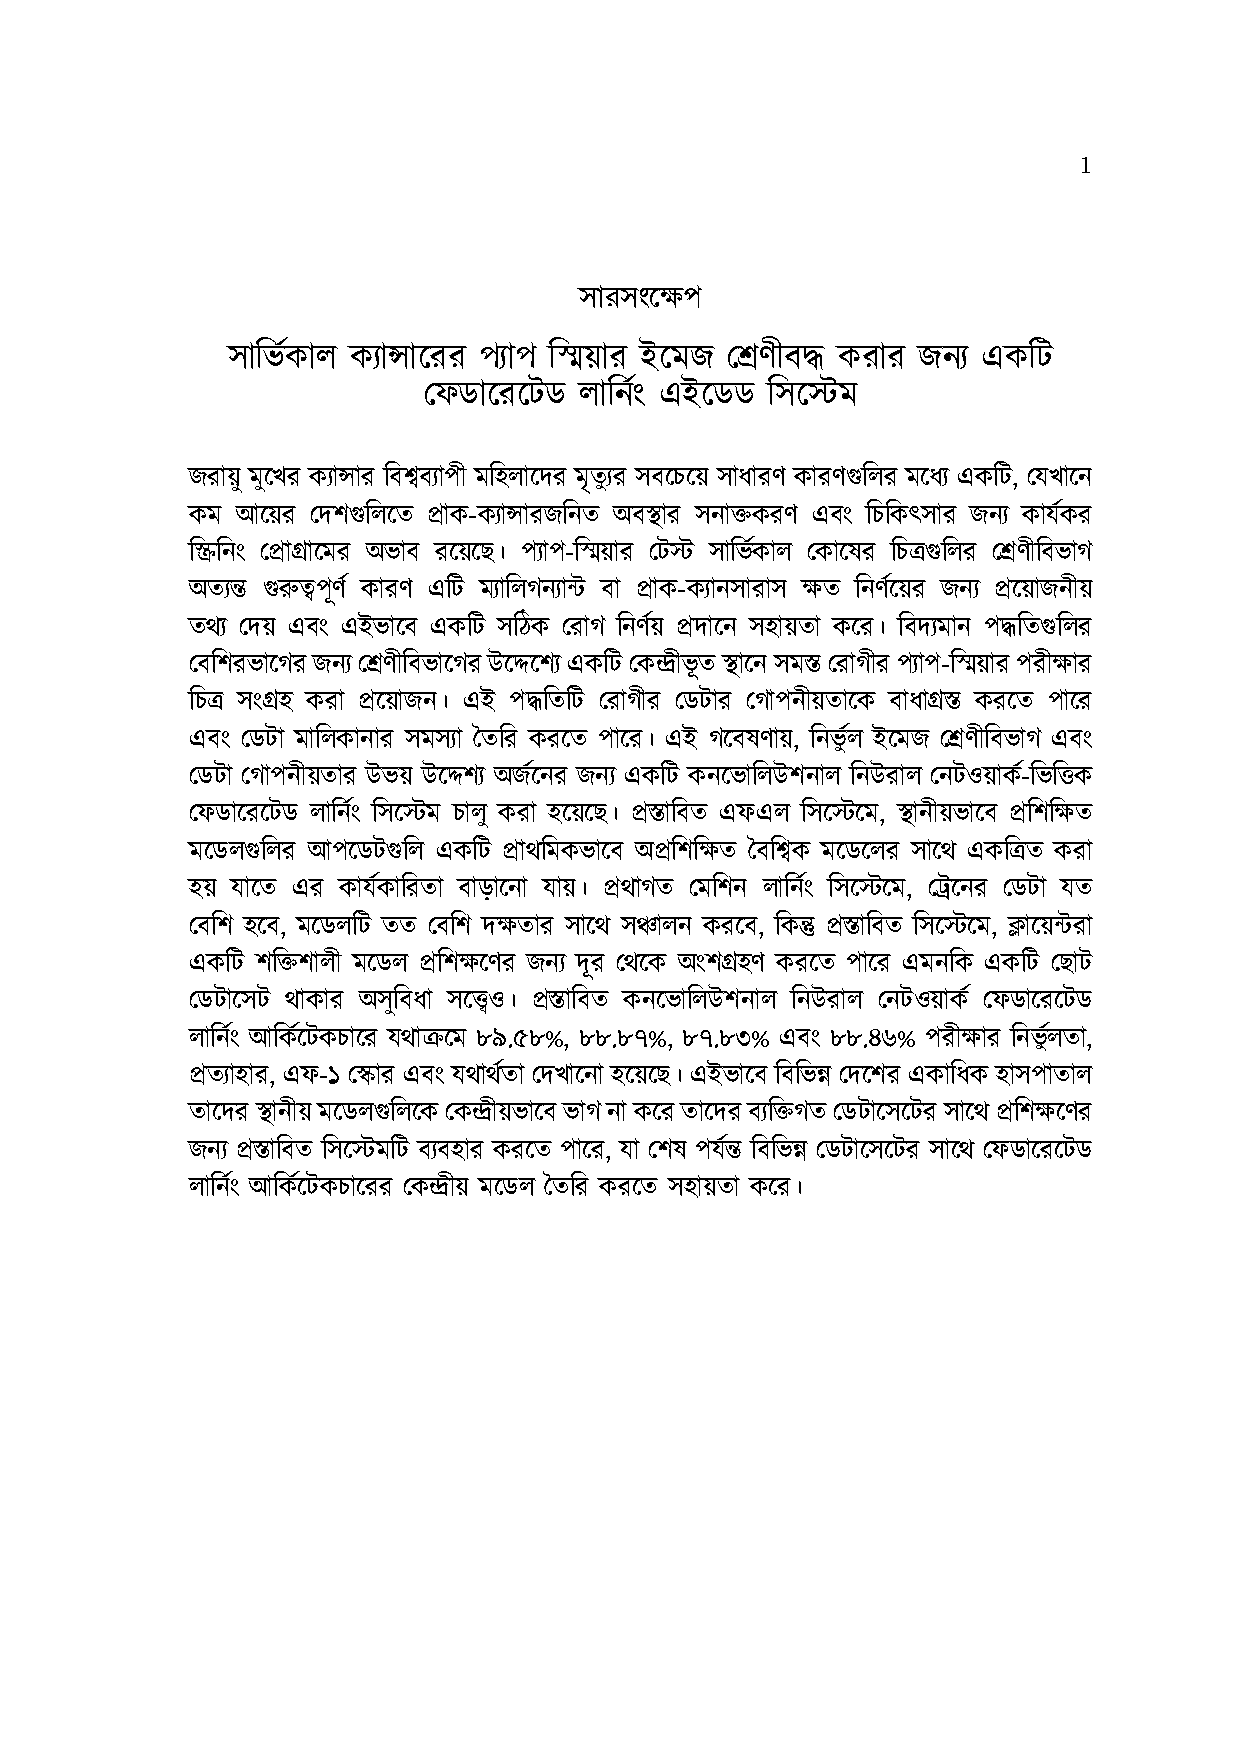
\includegraphics[height=10.7in, width=180mm, trim={32mm 0 0.5mm 4cm}, clip]{chapters/abstractBN.pdf}} 
    \end{center}
% 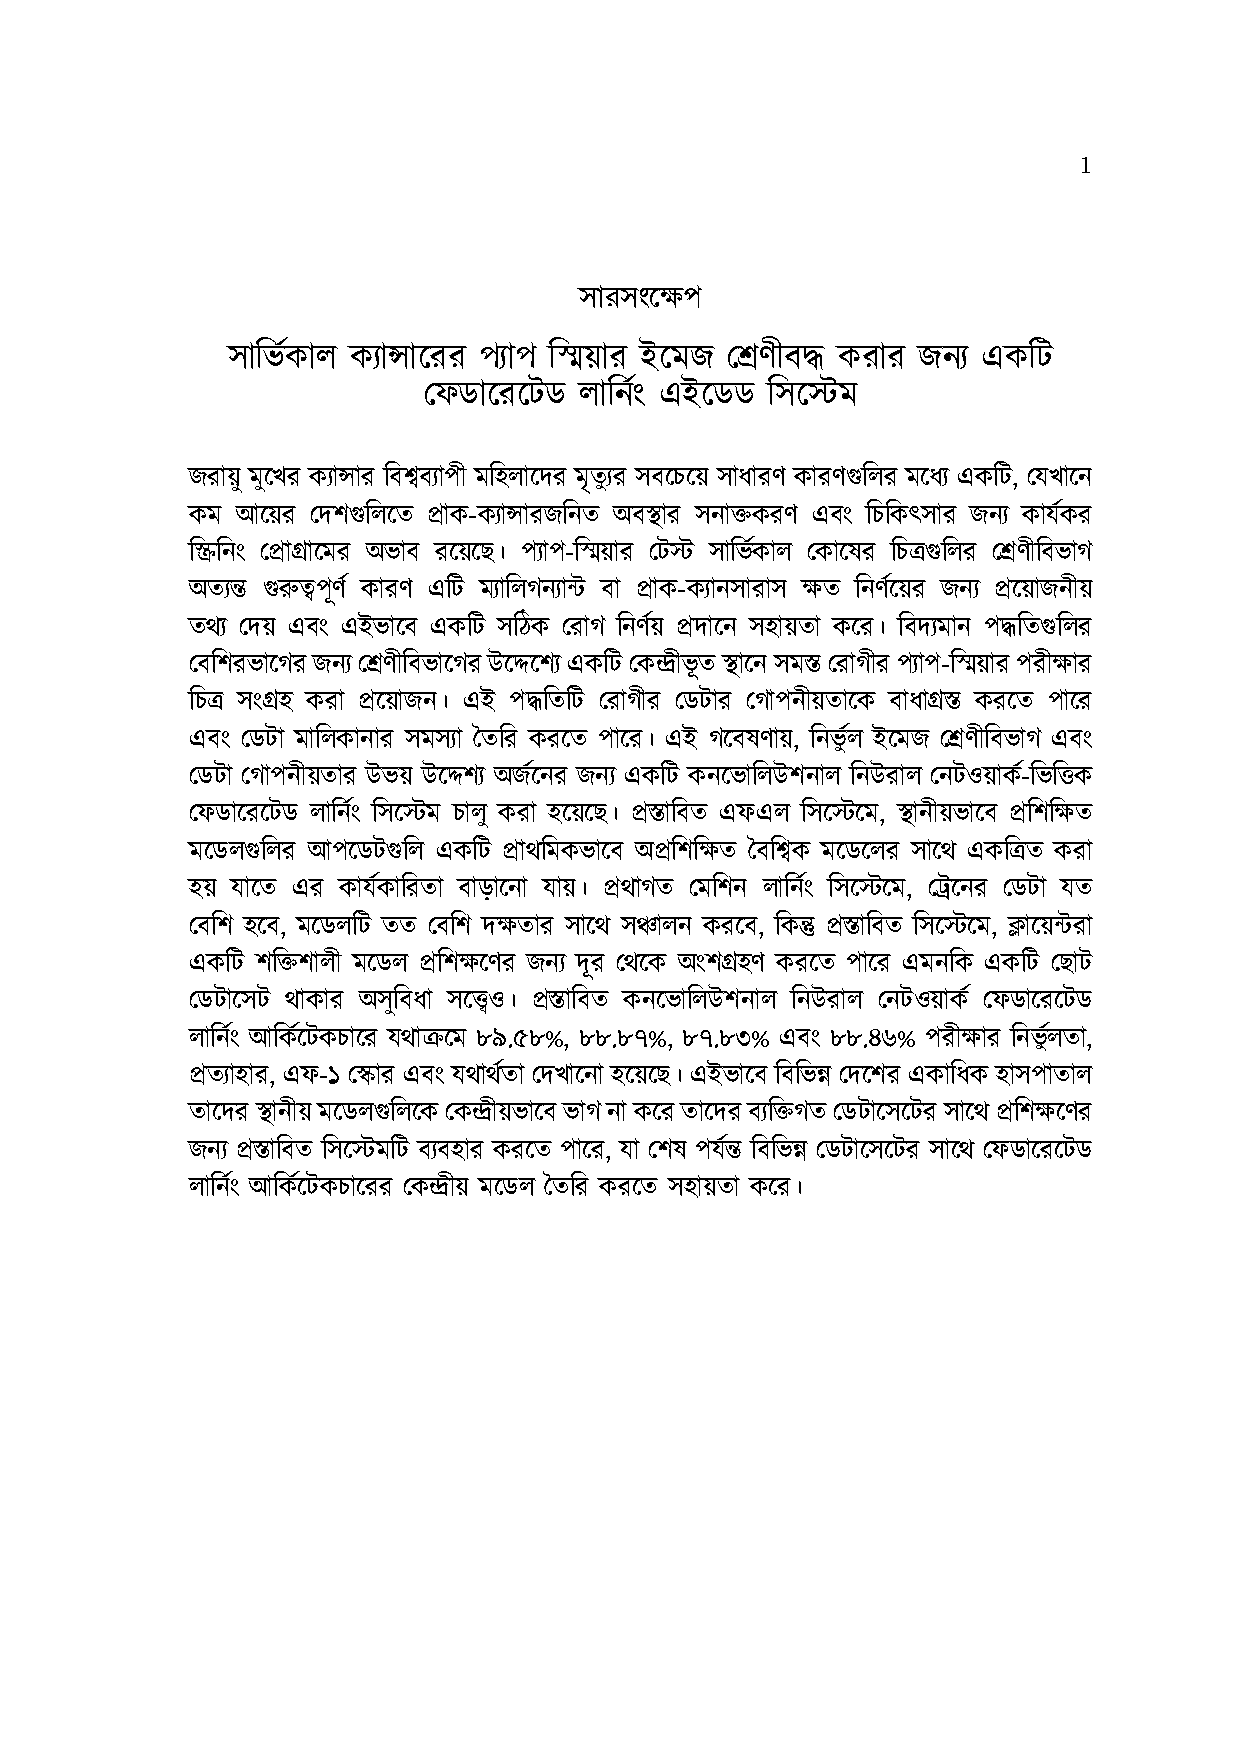
\includegraphics[height=10in, width = 165 mm]{chapters/abstractBN.pdf}
 

\noindent%



	% !TEX root = ../thesis.tex

\chapter{ACKNOWLEDGEMENTS}

\justifying
We are thankful to Almighty Allah for His blessings for the successful
completion of our thesis. Our heartiest gratitude, profound indebtedness and deep respect go to our supervisor, {\def\supdel{, }\endlinechar =-1\thesupervisor}, PhD, Supervisor, Associate Professor, Department of Computer Science & Engineering, and co-supervisor Nafiz Imtiaz Khan, Lecturer, Department of Computer Science and Engineering, Military Institute of Science and Technology
for their constant supervision, affectionate guidance and great encouragement and motivation. Their keen interest on the topic and valuable advices throughout the study was of great help in completing thesis. We are especially grateful to the Department of Computer Science and
Engineering (CSE) of Military Institute of Science and Technology (MIST) for providing their all out support during the thesis work.



Finally, we would like to thank our families and our course mates for
their appreciable assistance, patience and suggestions during the
course of our thesis.
%\vspace{1.25cm}
%\noindent
%{\hfill {\sc \theauthor}
%
%\smallskip
%\hfill {\it \theuniversity}
%
%\hfill {\it Dhaka, Bangladesh}
%
%\hfill {\it \theDefenseDate}}
%%\hfill {\it \monthname~2018}}


 






\vfill
%\end{acknowledgements}

	\ifdefined\theStudyType
	%list of abbreviations


%\chapter{listofabbreviations}
\chapter{LIST OF ABBREVIATIONS}
\noindent

%comment the lines below
%List all the alphabetically sorted abbreviations with the following latex command in the long table environment: 

%%Uncomment the below table environment to enter abbreviations.
%%--------------------------------------
%\begin{longtable}[l]{p{55pt}p{300pt}}
%%%\textbf{LSB}		&	Least Significant Bit\\
%%%\textbf{MSB}		&	Most Significant Bit\\
%\end{longtable}

%\end{listofabbreviations}

	\fi

	
	
	%************************************
	% Main Text
	\mainmatter{ 
		%\linespread{6}
		\doublespacing
		
		%--------------------------------
		% Chapter 1: Introduction
		\chapter{INTRODUCTION}
\label{chap1:intro}

%\begin{adjustwidth}{1.5cm}{0cm}
%\begin{myenv}{Chapter Organization}
%\small
%Summary of the chapter orientation may be added
%\end{myenv}
%\end{adjustwidth}
%\bigskip


%=============================================

This chapter puts forth a discussion on the background of the research, problem statement, objectives of the thesis, methodological overview, scope of the thesis and organization of the remaining chapters. It starts with describing the background of the research to give an insight into the problem statement and to demonstrate the objectives of the thesis. Then further details are introduced through the overview, scope and organization of the thesis.

\section{Research Background}

%=============================================
Cervical cancer is a type of cancer that develops in the cells of the lower portion of the uterus which connects to the cervix. The human papillomavirus (HPV), a sexually transmitted infection, is responsible for more than 95\% cases of cervical cancer. 
It may also be caused due to smoking, a weak immune system, birth control pills, having many sexual partners, etc. 

In 2020, there was a global estimation of 604,127 new cases and 341,831 deaths due to cervical cancer \cite{ar1}. With 569,847 new cases every year, cervical cancer has become the fourth most frequent disease afflicting women globally, after breast, colorectal, and lung cancers \cite{ar2}. In the context of Bangladesh, there are 58.9 million women, aged 15 years or older, are at risk of acquiring cervical cancer \cite{b1}. Each year 4971 women die from cervical cancer while 8268 women are diagnosed with it (estimations for 2020) \cite{b1}. Therefore the second most common malignancy in Bangladeshi women is cervical cancer \cite{b1}. 

Although no symptoms are visible during the early stages, some symptoms like vaginal bleeding, pelvic pain etc. are noticed later. Death due to cervical cancer can be reduced if effective screening strategies are implemented. Regular pap smear screening tests must be used to monitor women for early identification of cervical cancer so that effective treatment can be provided to the patients. For a proper diagnosis and the identification of malignant or precancerous lesions, it is crucial to classify cervical squamous cells according to their cytomorphology in Pap smear images \cite{ar3}.

Existing machine learning approaches to classify cervical cell images combine two or more datasets in order to increase the model's performance. 
But such publicly available datasets are few and far between. In order to harness the benefit of data privacy with the development of an effective deep learning model, researchers have applied FL for brain tumor segmentation and breast cancer histopathological image classification. But there is no research conducted for developing a differential privacy-enhanced FL system for cervical cell classification.

%=============================================
\section{Problem Statements}

%=============================================

In most of the existing methods, various machine learning and deep learning techniques have been introduced which require accumulating the pap-smear test images from different data resources in a centralized location for classification purposes. The more training data, the higher the model's accuracy. In the medical imaging domain, acquiring sufficient data is a significant challenge. Though this challenge could be addressed through collaboration between multiple institutions, sharing medical data in a centralized location faces various legal, privacy, technical, and data-ownership challenges. And also the institutions in possession of low amount of data can't achieve a satisfying performance from models trained with the existing methods.  

% For the classification of cervical cancer, we propose a CNN-based Federated Learning (FL) aided system. 

\clearpage
%=============================================
\section{Thesis Objectives}
\label{sec:objectives}
%=============================================
The primary goals that we want to achieve with this research are as follows: 
\begin{enumerate}
\item \textcolor{black}{To propose a novel Deep Learning architecture for the classification of cervical cancer cell images considering small datasets.}
\item \textcolor{black}{To integrate the best performed Deep Learning model with the FL architecture by evaluating them continuously using hyper-parameter tuning.}
\item \textcolor{black}{To develop a user-friendly and interactive web app for applying the proposed Federated Learning architecture in a real-world environment.}
\end{enumerate}
%=============================================
\section{Methodological Overview}
In order to meet the desired objectives, a literature review was conducted to gather knowledge from the previous research done on the topic. The study helps to gain better knowledge on the scope and uses of federated learning and to get a proper insight as to how the classification of Cervical Cancer can be done. It helps to know about the procedure of merging the data from different hospitals using federated learning to get an improved classification, without sharing of private data. Keeping this in mind, Federated Learning architecture was applied to a novel CNN model for the classification of cancer cells.

\section{Scope of the Thesis}
The study particularly focuses on the development of a web application, through which clients from different places can add their data, which would eventually aid in getting an accurate classification of the cancer cells. Here the main target is to update the global model periodically with the help of a variety of data collected from different institutions. The collaborating institutions can benefit from this system in several ways. 
\begin{enumerate}
    \item 
Federated Learning allows individual hospitals to address the challenge of possessing small dataset by collaborating with multiple non-affiliated hospitals. 
    \item 
Federated Learning utilizes diverse datasets of numerous collaborators for building a robust deep learning model.
    \item 
Federated Learning helps to classify the pap smear images of cervical cancer by aggregating locally trained model weights from different hospitals, referred to as “clients” to a centralized location model, known as the “server” model, without needing the clients to share their personal data. 

\end{enumerate}

% Thus, a FL-aided system can aid in the process of classifying pap smear images efficiently with the benefits of data privacy.

% The use of Federated Learning gives this advantage that data from any part of the world can be used to update the model, by ensuring privacy and avoiding the misuse of personal data. Each client uses their data to train the model, which helps to collect a variety of data. The collection of such diversified data eventually improves the overall classification process and thus would help in a better diagnosis


\section{Organization of Thesis}

The remaining chapters are organized as such: The theoretical background and the related work have been discussed in chapter 2. Firstly, a detailed discussion has been put forth about Cervical Cancer. Then the existing methodologies have been discussed. Finally, a critical appraisal is given.   
In chapter 3, a detailed description was provided of fifteen different traditional ML algorithms, Deep Learning and the process of Federated Learning. Federated Learning training algorithms: FedSGD and FedAvg were also discussed. The methodology which was carried out in this research is presented in Chapter 4. The process of system development has been discussed in chapter 5. This chapter is described using 3 subsections. The first subsection is about the acquisition of the dataset, the second subsection presents how the classical machine learning models have been developed and the results obtained from those models were analyzed. The final subsection describes how the architecture of federated learning is built from data partitioning, augmentation, foundation model development to prototype development for applying FL in a real-world environment. Thus the main purpose of this whole chapter is to give a brief discussion about the overall design of the system including the development of the base model. The ending chapter states the limitations and future works of thesis.

		%--------------------------------
		
		
		%--------------------------------
		%Chapter 2: Related Works
		\chapter{BACKGROUND THEORY AND RELATED WORK}
% \label{chap2-related-works}
This chapter is focused on the introduction of cervical cancer as well as previous research methodologies of detecting and classifying cervical cancer.
%====Chapter Summary START======
%\begin{adjustwidth}{1.5cm}{0cm}
%\begin{myenv}{Chapter Organization (optional)}
%\small
%Briefly describe the orientation of the chapters to give an initial idea to the reader.
%\end{myenv}
%\end{adjustwidth}
%\bigskip
%=====CHAPTER SUMMARY END=======


% \label{chap2sec:introduction}

\section{Cervical Cancer}

Cervical cancer occurs within the cells of the cervix. The cervix is the slender end of the uterus that forms a connection between the uterus and the birth canal. Before the appearance of cancer in the cervix, the cells of the cervix undergo such a change, in which abnormal cells are found to appear in the cervical tissue. These abnormal cells may turn to cancer cells over time, if not destroyed or removed. The cancer cells then start to grow and spread deeper into the cervix, as well as the surrounding areas. The two main types of cervical cancer are Squamous cell carcinoma and Adenocarcinoma. To detect the type and to know how far cervical cancer has spread, cell images have been divided into 5 categories here. The categories considered are Dyskeratotic, Koilocytotic, Metaplastic, Parabasal, and Superficial-Intermediate. The Dyskeratotic cells are the type of squamous cells that underwent premature abnormal
keratinization within individual or clusters of cells. The presence of dyskeratocytes in cervical smears may be predictive of either a simultaneous HPV infection or an infection the Koilocytotic cells are mostly the mature squamous cells, and Metaplastic cells are small or large parabasal cells with prominent cellular borders which may contain large intracellular vacuole, Parabasal cells are the immature squamous cells which are the smallest epithelial cells, Superficial-Intermediate cells show morphological changes
which indicate more severe lesions. This classification would help to know better about the severity and thus offer a better treatment accordingly.


\section{Related Works for Cervical Cancer Classification}

For the purpose of detecting cervical cancer, researchers employed three distinct classifiers: Softmax regression (SR), Support vector machine (SVM), and GentleBoost ensemble of decision trees (GEDT) \cite{ar4}. Over a convolutional neural network, they suggested using these three to create an autonomous cervical cancer detection system. They came to the conclusion that, when compared to the other strategies stated, the proposed system appeared to perform better and produced the maximum performance. 

For the first time, federated learning was presented in a study on the modality of cardiovascular magnetic resonance (CMR), with four centers derived from subsets of the MM and ACDC datasets, focusing on the diagnosis of hypertrophic cardiomyopathy (HCM) \cite{ar5}. They modified a 3D-CNN network that had previously been trained on action recognition and investigated two approaches to incorporating shape prior information into the model, as well as four different data augmentation setups, systematically analyzing their impact on the various collaborative learning options. Despite the small sample size (180 subjects from four centers), they demonstrated that privacy-preserving federated learning achieves promising results that are competitive with traditional centralized learning. They also discovered that federatively trained models are more robust and less susceptible to domain shift effects. 

Federated learning enabled deep learning model was used on multimodal brain scans \cite{ar6}. The quantitative results show that federated semantic segmentation models (Dice=0.852) perform similarly to models trained by sharing data (Dice=0.862). The comparison was shown among federated learning and two other collaborative learning methods and it concluded that these methods fall short of the performance of federated learning. 

 A Federated learning-based cancer diagnosis model was proposed where six first-level impact indicators were identified, as well as historical case data from cancer patients \cite{ar7}. In the federated learning framework combined with the convolutional neural network, various physical examination indicators of patients were used as input. An auxiliary diagnostic model was built using patients’ recurrence time and location, and comparison algorithms included linear regression, support vector regression, Bayesian regression, gradient ascending the tree, and multilayer perceptrons neural network. CNN’s federated prediction model based on improved accuracy under the condition of joint modeling and simulation on the five types of cancer data accuracy reached more than 90. 

In a study conducted by Pati et al. \cite{ar8}, The most extensive real-world FL effort to develop an accurate and generalizable ML model for detecting glioblastoma subcompartment boundaries was described in a research. Notably, the study’s collaborators’ extensive global footprint yields the largest dataset ever reported in the literature assessing this rare disease. FL provided unprecedented access to the most common and fatal adult brain tumor dataset, as well as meaningful ML training to ensure model generalizability across out-of-sample data. Because FL enabled large and diverse data, the final consensus model outperformed the public initial model against both the collaborators’ local validation data and the entire out-of-sample data.

In another study, the feasibility of using differential-privacy techniques was investigated to protect patient data in a federated learning setup \cite{ar9}. They developed and tested practical federated learning systems for brain tumor segmentation on the BraTS dataset. The experimental results revealed that there is a tradeoff between model performance and privacy protection costs. 

How data dispersion affects FL performance was outcome of a research \cite{ar10}. The two parts of their proposed system, bag preparation and Multiple-Instance Learning, were local to each client (MIL). The authors explored the possibility of learning from distributed medical data via differentially private federated learning. They mainly showed how FL might be utilized in clinical contexts to guarantee data privacy while also ensuring minimal performance reduction. 

One study gave an outline of how federated artificial intelligence can be used in medical imaging applications while maintaining security and privacy \cite{ar11}. They talked about how AI has changed the area of medicine, what is needed for the best privacy preservation, and the privacy and security concerns with medical imaging. 

The study of Ghoneim, Muhammad, \& Hossain showed the development of a cervical cancer categorization and detection method based on CNN \cite{ar12}. Three CNN models and an ELM-based classifier were studied. The shallow CNN model was trained and tested using the 5-fold cross-validation method on the Herlev dataset from the database. They concluded by demonstrating how the ELM-based classifier produced a greater accuracy than all the other methods. 

The use of hybrid pipelines for the detection and classification of aberrant regions in liquid-based cytology (LBC) pictures using a combination of deep learning (DL) and traditional machine learning (ML) techniques was demonstrated in another study \cite{ar13}. They made use of a personal database containing 1920 x 2560 pixel photos. They demonstrated how to inspect cervical samples using a RetinaNet model for the detection of aberrant regions. 

A pre-trained CNN architecture was used along with a support vector machine for the detection of Cervical Cancer \cite{ar14}. For the pre-trained architecture, the AlexNet was used to extract the desired features and showed how it performs better with better recall, precision, specificity and accuracy scores than other compared techniques. 

In another research, the Herlev and SIPaKMeD datasets were integrated for the purpose of detecting cervical cancer. They demonstrated their ability to successfully analyze multi-layer cervical cells and developed a binary and multi-class classification pipeline to identify cancer in Pap smear images  \cite{ar15}. 

 A focused study included reviews of the various cervical cancer diagnostic techniques \cite{ar16}. They called attention to the flaws and limitations of the analytical techniques and procedures. They made the observation that subpar preprocessing and segmentation resulted in subpar classification outcomes.

The main discoveries made from the study include:
\begin{enumerate}
    \item
    Except some recent works, very few such instances of incorporation of Federated Learning in the classification of cervical cancer cells are available.
    \item
    Most previous attempts of classification are methods which require data sharing which eventually hampers privacy.
    \item
    Most existing systems do not show concern for the development of a personalized Convolutional Neural Network model for the purpose of classification.
\end{enumerate}


\section{Critical Summary}

In order to protect patient data privacy and produce reliable findings even with the drawback of limited data, federated learning is necessary in a variety of illness prediction and classification systems. This technique has already been used in the diagnosis of hypertrophic cardiomyopathy, the segmentation of brain tumors, the prediction of breast cancer, and many other things. A decentralized machine learning method called federated learning enables several parties to train a machine learning model without disclosing their personal information. This method has a great deal of potential in the healthcare industry, where data privacy is a major problem.

Without actually sending the data to a central server, federated learning can be utilized in the healthcare industry to train models on private patient information. This can support patient privacy protection while yet allowing for medical research and individualized care. Healthcare fields including disease prediction, medication research, and clinical decision-making can all benefit from federated learning.

The creation of a model to forecast diabetic retinopathy, the main cause of adult blindness, is one instance of federated learning in the healthcare industry. Without releasing the data directly, researchers trained the model using data from many hospitals using a federated learning approach. This method produced a very accurate model while preserving data privacy.

Ultimately, federated learning has the potential to transform healthcare by facilitating more individualized medical research and treatment while protecting patient privacy. The standardization of data across many hospitals and ensuring the stability and dependability of the federated learning models are two obstacles that must yet be overcome.

		%--------------------------------
		
		%--------------------------------
		% Chapter 3: My Work/contribution
		\chapter{THEORETICAL BACKGROUND}
\label{chap3:background}

The theoretical background defines a variety of subjects, including traditional machine learning methods, deep learning methods, federated learning concepts for training the model to classify the cervical cell images and other relevant concepts.

\section{Traditional Machine Learning Algorithms}

\subsection{LightGBM}
Light Gradient Boosting Machine or, LightGBM is a highly efficient Gradient boosting decision tree, which provides increased accuracy and efficiency. It is a gradient boosting framework that utilizes tree based learning algorithms. It has the advantages like capability of handling larger scale data, better accuracy, decreased memory usage, etc. LightGBM splits the tree leaf-wise in order to ensure lower loss. 

\begin{figure}[H]
\centering
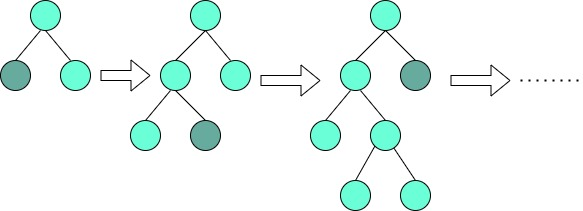
\includegraphics[width=150mm,height=50mm]{figures/lgbm.jpg}
\caption{Leaf-wise tree growth used in LightGBM}
\label{DLAccuracy}
\end{figure}


The LightGBM algorithm utilizes two novel techniques called Gradient-Based One-Side Sampling (GOSS) and Exclusive Feature Bundling (EFB) which allow the algorithm to run faster while maintaining a high level of accuracy \cite{ar22}.

\subsection{Histogram Gradient Boosting With LightGBM}
In order to speed up the Gradient boosting decision tree (GDBT) process,using histogram proves to be an important technique \cite{ar23}. To ensure better quality in less inference time, an advanced base learner called piecewise linear tree is utilized.

\begin{figure}[H]
\centering
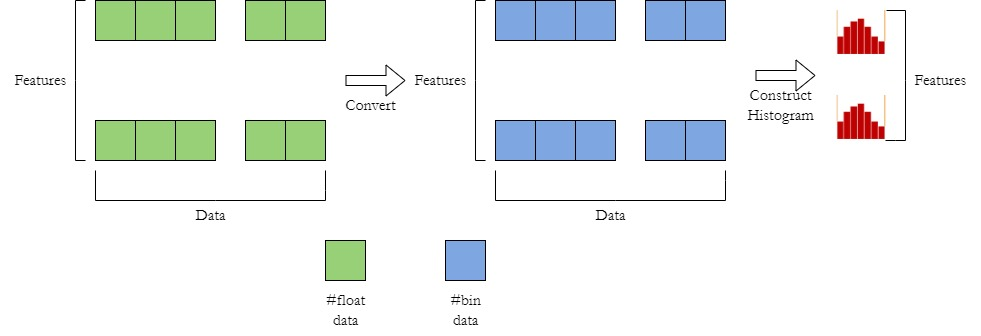
\includegraphics[width=160mm,height=55mm]{figures/hgb_lgbm.jpg}
\caption{Histogram Algorithm of LightGBM}
\label{DLAccuracy}
\end{figure}

\subsection{Histogram Gradient Boosting}
Histogram Boosting was released by Scikit-Learn, which was named as HistGradientBoostingClassifier. Its operation is similar to that of LightGBM, but offers a much faster speed than gradient boosting. It provides built in support for the missing values, and is used for faster training of decision trees.  

\subsection{Xtra Trees}
Extremely randomized trees or extra trees is an ensemble supervised machine learning method. The extra trees algorithm works by creating multiple decision trees, where the sampling for each tree is done randomly. Thus the dataset taken for each tree is made with unique samples. To output the classification result, it aggregates the results of the multiple de-correlated decision trees, which are collected in a "forest". Thus it holds similarity to the Random Forest Classifier, but differs with respect to the construction of the Decision Trees in the forest.

\subsection{SVM}
Support Vector Machine (SVM) is a machine learning method which helps to largely overcome the curse of dimensionality and other issues faced while applying the traditional learning methods. SVM takes the optimal separating hyperplane as the decision surface, which is able to classify two classes of data while maximizing the distance between the points \cite{ar24}.  Thus all of the data points on one side of the hyperplane will represent one category and the data points on the other side of the hyperplane will represent a different category. Support vector machines are a set of supervised learning methods, that can be used to detect cancerous cells, on the basis of millions of cells.

\subsection{SVM Grid Search}
SVM has some hyper-parameters, and the optimal one can be found by creating a grid of hyper-parameters and just try all the possible combinations. This approach taken is termed as Grid Search. In the Grid Search method, all the possible combinations of hyperparameters will pass one by one into the model and check each model's score. As a result, it gives us a set of hyperparameters which give the best possible score.  Grid Search calculates the error for various hyperparameter values, and eventually aids in choosing the best values.

\subsection{Gradient Boosting}
Gradient boosting is a machine learning technique that is used in both regression and classification tasks. It gives a prediction model in the form of an ensemble of weak prediction models, which are typically decision trees. It is termed as a sequential ensemble learning technique, as the performance of the model is found to improve over iterations. In this case a group of weak prediction models, like regression decision trees, are modeled by adding new learners in a sequential manner. It can give prediction results based on the decision nodes, and can provide an improved accuracy when viewed as an ensemble \cite{ar25}. 

\subsection{XGBOOST}
Extreme Gradient Boosting or XGBoost also uses a gradient-boosting based approach in order to ensure optimization in the tree split against a predefined loss function.  It is an ensemble learning method which combines the predictions of multiple weak models to produce a stronger prediction. XGBoost has the advantage that it can deal with any missing data, unlike other ML models that require additional processing on the training data. It does not require an immense set of pre-processing operations and thus minimizes the communication costs significantly and also reduces the leakage of  private data \cite{ar26}. 

\begin{figure}[H]
\centering
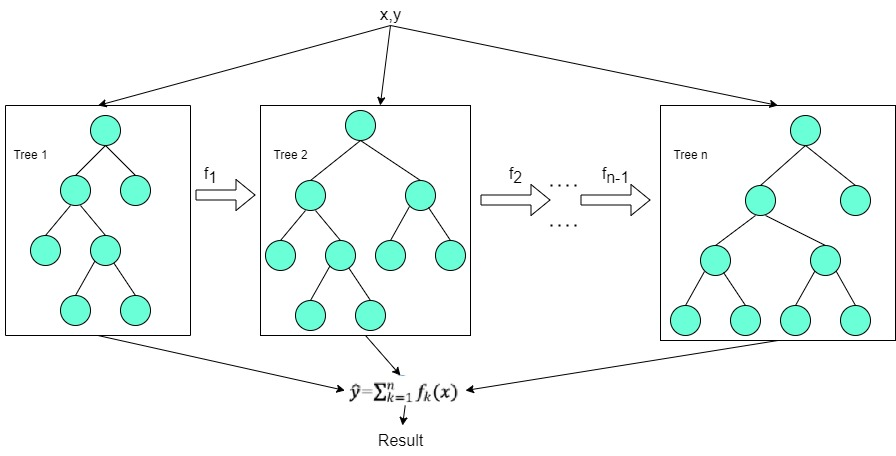
\includegraphics[width=150mm,height=70mm]{figures/xgb.jpg}
\caption{A General Architecture of XGBoost}
\label{DLAccuracy}
\end{figure}

XGBoost has a wide range of hyperparameters that can be adjusted to optimize performance, making it highly customizable and also provides feature importances, which helps in making important predictions.

\subsection{MLP}
A multilayer perceptron (MLP) is a fully connected class of feedforward artificial neural network (ANN). The multilayer perceptron can be trained to approximate virtually any measurable function, as it does not make any prior assumption regarding the data distribution. The multilayer perceptron can model the non-linear functions, and can also be trained so that whenever presented with any unseen data, it can accurately generalise the information \cite{ar28}. The multilayer perceptron is a system of interconnected neurons, consisting of input and output layers, and one or more hidden layers.

\begin{figure}[H]
\centering
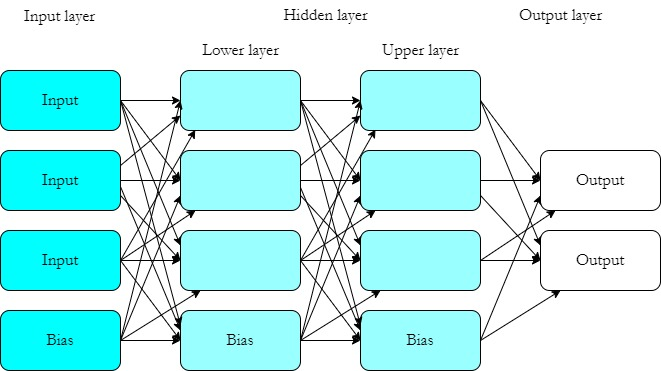
\includegraphics[width=125mm,height=70mm]{figures/mlp.jpg}
\caption{The multilayer perceptron}
\label{DLAccuracy}
\end{figure}

\subsection{Histogram Gradient Boosting With XGBoost}
Histograms can be applied to the Extreme Gradient Boosting, or XGBoost for the continuous input variables. It eventually helps to provide a highly optimized implementation of gradient boosting.

\subsection{KNN}
K-Nearest Neighbor or KNN Algorithm is a non-parametric, supervised learning classifier, which makes use of approximation to make classifications about the grouping of an individual data point. It can be used for both regression and classification, but it is mostly utilized in classification algorithms. The average of the k nearest neighbors is considered to make a prediction about the classification of a new data point. For this, the K-NN algorithm assumes the similarity between the new data and all the available data and places the new data into the category which is most similar to the available categories.

\begin{figure}[H]
\centering
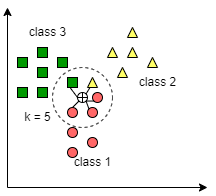
\includegraphics[width=95mm,height=75mm]{figures/knn.png}
\caption{K Nearest Neighbours}
\label{DLAccuracy}
\end{figure}

KNN is a non-parametric algorithm, as it does not make any assumption regarding the underlying data. It is sometimes termed as a lazy-learner as it does not learn anything from the training set immediately. It merely stores the dataset and performs an action on it at the time of classification.


\subsection{Decision Tree}
A decision tree is a decision support tool that uses a tree-like model, made up of decisions and their possible consequences. An instance is classified by starting at the root node of the tree, then it gradually moves down until it reaches the leaf. The internal nodes denote a test on an attribute. Drawn from left to right, the contents of the leaf node represent the outcome of the decisions. The decision tree follows a non-parametric approach, which means that it is distribution-free and does not depend on the assumptions of probability distribution. It can operate on any high-dimensional data with exceptional accuracy.

\begin{figure}[H]
\centering
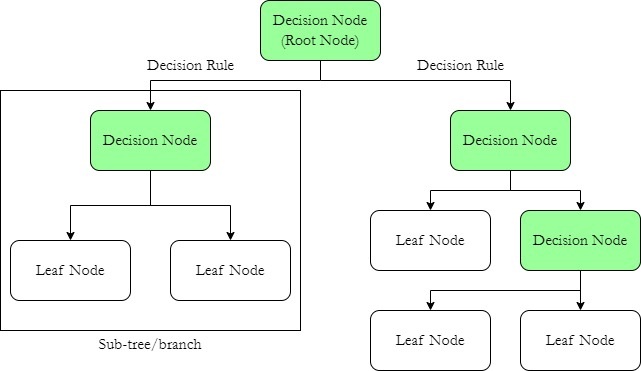
\includegraphics[width=130mm,height=80mm]{figures/dt.jpg}
\caption{Decision Tree Classifier}
\label{DLAccuracy}
\end{figure}

\subsection{AdaBoost}
AdaBoost or Adaptive Boosting is a method in machine learning, which is used as an ensemble learning  method. A strong model can be built by grouping multiple weak classifiers where each one gets to progressively learn from the others' wrongly classified objects. The multiple weaker models are independently trained and their predictions get combined to make the overall prediction.

% \begin{figure}[H]
% \centering
% 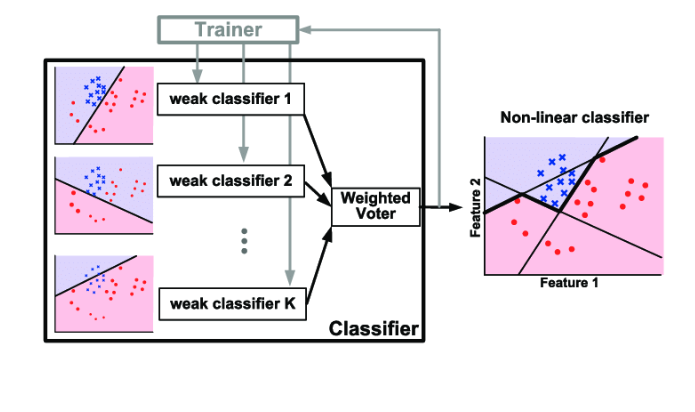
\includegraphics[width=90mm,height=38mm]{figures/adaboost.png}
% \caption{AdaBoost algorithm for creating a strong classifier based on multiple weak linear classifiers.}
% \label{DLAccuracy}
% \end{figure}

% The application of  algorithms in order to create a strong classifier is shown in fig …. 

Boosting is a machine learning technique used for both regression and classification problems. It produces a prediction model which holds characteristics which represent an ensemble of weak prediction models, typically decision trees. It builds the model in a gradual manner, like other boosting methods do. It generalizes the models by allowing optimization of an arbitrary differentiable loss function (\cite{ar27}).

\subsection{Random Forest}
are ensemble learning techniques for classification, regression, and other problems that work by building a large number of decision trees during the training phase The class most trees choose in a classification problem is the output of the random forest.

\subsection{Gaussian Naive Bayes}
It is an extension of the Naive Bayes Algorithm. Gaussian Naive Bayes is a classification technique, which is used in Machine Learning (ML) based on the probabilistic approach and Gaussian distribution. This algorithm does not need much time for training and gives results which are greatly reliable. 

\section{Deep Learning}
Artificial neural networks, a class of algorithms inspired by the structure and operation of the brain, are the focus of the machine learning discipline known as deep learning. Some of the data pre-processing that is generally involved with machine learning is eliminated with deep learning. These algorithms can handle text and visual data that is unstructured and automate feature extraction, reducing the need for human specialists. 

The process of recognizing photographs and classifying them into one of several predetermined different categories is known as image recognition (or image classification). As a result, image recognition software and apps can identify the objects in a photo and differentiate one from another. Computer vision is the branch of study that aims to give machines this capability. Deep learning models can be used by researchers to solve computer vision problems.

Deep learning systems need access to enormous amounts of training data and processing power in order to attain an acceptable degree of accuracy. Until the age of big data and cloud computing, neither of these resources was readily available to programmers. Deep learning is able to produce precise predictive models from enormous amounts of unlabeled, unstructured data because it is capable of producing complicated statistical models directly from its own iterative output. 

\subsection{CNN}
A Convolutional Neural Network (ConvNet/CNN) is a Deep Learning algorithm that can take in an input image, give importance (learnable weights and biases) to various aspects in the image, and be able to distinguish one from the other. In comparison to other classification methods, a ConvNet requires significantly less pre-processing. ConvNets have the capacity to learn these filters and properties, whereas in basic techniques filters are hand-engineered.

The structure of a ConvNet was influenced by the way the Visual Cortex is organized and is similar to the connectivity pattern of neurons in the human brain.

\subsection{Layers of CNN}
Convolutional Neural Networks (CNNs) are constructed from layers that perform different operations on the input data. The primary layers used to construct a CNN are as follows:

\subsubsection{Convolutional layer}
To perform the convolution process, a convolutional layer applies a number of learnable filters or kernels to the input image or feature map. A set of feature maps that represent different aspects of the input picture or feature map make up a convolutional layer's output. Let K be the kernel detector and I be the image used as the input. The output feature map O can then be created by convolving the input image with the kernel and using an activation function, similar to what was done in 3.1:

\begin{equation}
\label{eq:cnn_conv_layer}
    \textcolor{black}{O(i,j) = f(\sum\sum I(m,n) * K(i-m,j-n)}
\end{equation}

where f denotes the activation function, (i,j) denotes a location in the output feature map, and (m,n) denotes the location of the input image pixel that the kernel is now aligned with. The whole feature map can be retrieved by swiping the kernel over the full input image.

\subsubsection{Activation Layer}
An activation layer applies a non-linear activation function to the output of a fully connected layer or a convolutional layer.

Let X be the input (which is often the output of a convolutional or fully connected layer) and f be the activation function for the activation layer. Each element of the input X is subjected to the activation function by the activation layer, which results in the output Y. As seen below, the output Y is calculated:

\begin{equation}
\label{eq:activation_layer}
    \textcolor{black}{Y(i,j,c) = f(X(i,j,c)}
\end{equation}

where i, j, and c are the input and output tensors' spatial and channel coordinates. Sigmoid, tanh, and ReLU (Rectified Linear Unit) activation functions are frequently used in CNNs. The precise requirements of the work and the type of data being processed dictate the activation function to be used.

\subsubsection{Pooling Layer}
A pooling layer reduces the spatial size of feature maps while retaining the most crucial data. The two most used pooling operations are average pooling, which chooses the average value from each patch of a feature map to produce a smaller map, and max pooling, which returns the maximum value inside a pooling window. The following mathematical diagram illustrates how pooling works:
Let P represent the pooling size, S represent the stride, and F represent the input feature map. The output feature map O can then be created by pooling the input feature map with a pooling window of size P and a stride of S:

\begin{equation}
\label{eq:pooling_layer}
    \textcolor{black}{O(i,j) = Pooling(F(iS : iS+P,jS : jS+P)}
\end{equation}

% O(i,j) = Pooling( F(iS : iS+P, jS : jS+P) )

where Pooling is a pooling function that produces a single value from values in the pooling window.

\subsubsection{Batch Normalization Layer}
The layer of batch normalization enables the network's layers to learn more independently. The output of the earlier layers is normalized using it. In normalization, the activations scale the input layer. Learning becomes more effective when batch normalization is utilized, and it can also be used as regularization to prevent model overfitting. To standardize the input or the output, the layer is added to the sequential model. It can be applied in a number of places between the model's layers. It is frequently positioned immediately after the convolution and pooling layers and after specifying the sequential model.

\subsubsection{Dropout}
The regularization method used to stop overfitting in the model is called dropouts. A certain percentage of the network's neurons are switched at random with the addition of dropouts. The incoming and outgoing connections to the neurons are also turned off when they are turned off. To help the model learn more effectively, this is done. Dropouts are typically advised against using them after convolution layers; instead, they should be utilized after the network's dense layers. It is always advisable to turn off the neurons just to 50\%. There is a possibility that the model leaning and the forecasts would be poor if we turned off more than 50\%.

\subsubsection{Flatten Layer}
A flattened layer transforms a 2D or 3D feature map into a 1D vector that can be used as input to fully connected layer. 
Let F be the input feature map of size H x W x C, where H is the height, W is the width, and C is the number of channels. Concatenating the rows of the feature map will then yield the flattened vector F':

\begin{equation}
\label{eq:flatten_layer}
    \textcolor{black}{F' = [F(1,1,1), F(1,2,1), ..., F(1,W,1), F(2,1,1), ..., F(H,W,1), F(1,1,2), ..., F(H,W,C)]}
\end{equation}

% F' = [F(1,1,1), F(1,2,1), ..., F(1,W,1), F(2,1,1), ..., F(H,W,1), F(1,1,2), ..., F(H,W,C)]

where the value of the feature map at position (i,j) in channel c is represented by F(i,j,c). The 2D or 3D feature map is flattened into a 1D vector using the equation above, which may then be utilized as input to a fully connected layer or other kinds of layers in the neural network.

\subsubsection{Fully Connected Layer}
The flattened feature vector serves as the fully connected layer's input, and a group of class scores serves as its output. Neurons in the layer that is entirely interconnected are coupled to each and every neuron in the layer below it. Generally, the output of the fully connected layer is fed into a softmax layer, which converts class scores into a probability distribution across classes.

\subsection{Activation Function}
An activation function is a mathematical function that deep neural networks employ to introduce nonlinearity into a layer's output. The use of activation functions is used to achieve this. It is used to change a layer's output into a more complex representation, allowing the network to learn complex and non-linear relationships between the input and the output. The ReLU activation function is applied following each convolutional layer in any CNN. As a result, the layer's output is effectively made non-linear, allowing the network to learn intricate details from the input images.

The activation functions Sigmoid, Tanh (Hyperbolic Tangent), and Leaky ReLU are frequently employed in deep learning. Based on the features of the data and the nature of the problem being addressed, the activation function is chosen.

\subsubsection{ReLU (Rectified Linear Unit):}
Deep neural networks frequently use the ReLU activation function since research has shown that it enhances the training of deep models. Any negative input is translated to 0, while positive inputs are left unaffected. The ReLU function is described as:

\begin{equation}
\label{eq:relu}
    \textcolor{black}{f(x) = max(0, x)}
\end{equation}
% $f(x) = max(0, x)$
The activation function's input in this case is 'x'. The ReLU function's output is almost always non-negative. The ReLU function's output is equal to the input when the input is positive. The output of the ReLU function is zero when the input is negative. ReLU is frequently used as the activation function in a neural network's hidden layers, while sigmoid is frequently utilized as the activation function in the output layer for binary classification tasks.

\subsubsection{Sigmoid:} 
For binary classification tasks, the sigmoid activation function is frequently used. All real-valued input is converted to a value between 0 and 1, which can be thought of as a probability. The sigmoid function is described as:

\begin{equation}
\label{eq:sigmoid}
    \textcolor{black}{f(x) = \frac{1}{(1+e^{-x})}}
\end{equation}
% $f(x) = \frac{1}{1+e^{x}}$
In this case, the activation function's input is 'x'. The sigmoid function's output has an inflection point at x = 0, and it always ranges between 0 and 1. The sigmoid function's output gets closer to one when the input is positive. The output of the sigmoid function gets closer to zero when the input is negative.


\section{Federated Learning}
\subsection{Federated Learning Mechanism}
Federated Learning is a collaborative machine learning technique where multiple edge devices(clients) participate remotely to train a common, robust machine learning model (server) without exchanging/sharing their local data samples with the centralized location or server which helps organizations to make better decisions with AI, addressing critical issues of data privacy, security, access rights and access to heterogeneous data.

\subsection{Traditional ML Vs. Federated Learning}
Traditional machine-learning approaches require a centralized location i.e. a single server to aggregate user data and carry out the complete training process, whereas federated learning allows continuous training on edge devices while ensuring no sensitive information exits the device. In the classical machine learning model, it is quite common to assume that the data are independent and identically distributed. On the contrary, federated learning assumes the data to be non-i.i.d because in real-world circumstances, various users have different datatypes and the expected and actual number of actors varies.

\subsection{Data Partitioning}
There are 3 types of data partitioning systems in federated learning: horizontal data partitioning, vertical data partitioning and federated transfer learning system. The description of the these 3 types is given below:

\textbf{1. Horizontal Data Partitioning :}
In horizontal partition, each edge device has overlapping features with different observations. For instance, if multiple hospitals in various countries collect data on breast cancer patients but have little to no overlapping of patients, that distribution is horizontal partitioning \cite{ar17}. 
		
\textbf{2. Vertical Data Partitioning :}
In the vertical partition, each device has different features with overlapping observations. For example, if a hospital suggests patients to a specific surgeon, both the hospital and the surgeon collect different kinds of data but will have many common patients \cite{ar17}.

\textbf{3. Federated Transfer Learning :}
If there are a few similar samples with few similar features, but also samples and features do not overlap, then federated transfer learning can be applied in this situation \cite{ar17}.

\subsection{Foundation ML model}
Depending on real-life scenarios, limitations of available datasets and problem statements, different kinds of ML models are decided to be used as the foundation model of federated learning architecture. Neural networks, decision trees, and even linear models are used on basis of use cases. This base model serves as a global model which is initially distributed as an untrained or pre-trained model from a central server to the local clients. The clients then collaboratively train the global model by continuously improving it in every communication round between the central server and the local clients. 

\subsection{Communication Architecture}
There are two types of FL communication architecture: centralized and decentralized. Both types of architecture work similarly; the distinction between them is in client-server communication. 

\textbf{1. Centralized Federated Learning :}
In a centralized federated learning system, a single central server is used, so there is only one possible point of failure \cite{ar19}.  In a centralized federated learning environment, a central server is utilized to manage all the participating nodes and orchestrate the various steps of the algorithms. The server is in charge of selecting the nodes at the start of the training process and aggregating the received model parameter updates. The server can end up being the system's bottleneck because each of the chosen nodes must communicate updates to the server \cite{ar18}. 

\textbf{2. Decentralized Federated Learning :}
Decentralized federated learning does not rely on a single central server to provide updates, in contrast to centralized federated learning \cite{ar19}. In this architecture, the nodes can collaborate among themselves to produce the global model. As the model updates are solely transferred between linked nodes without the coordination of a central server, this configuration avoids single-point failures \cite{ar21}. 

\subsection{Scale of Federation}
Federated learning can be divided into two categories based on the participating clients and the model training scale: cross-device FL and cross-silo FL \cite{ar20}.

\textbf{1. Cross-silo}: Cross-silo FL, where clients are organizations or companies and the client number is typically low (e.g., within a hundred) \cite{ar20}. 

\textbf{2. Cross-device}: Cross-device, where clients are typically mobile devices and the client number can reach millions \cite{ar20}. 


\subsection{One Federated Round}
The step where each participant completes training their local model and sends their model weights to the server so the server can combine their global model with the recently updated parameters of local models is referred to as a single communication round between the server and participant clients.

\subsection{Participants of the network}

There are two types of participants in a single federated round :
\begin{itemize}
    \item Client devices: These are the local devices that participate in the federated learning process by sending the updated weights of their locally trained models to the server.
    \item Server: The server uses the federated learning process by aggregating the model weights received from the client devices and sending the averaged weights back to the local devices for further training and to improve their accuracy.
\end{itemize}

\subsection{Process}

In a single federated round, the following steps are completed one after another: 
\begin{enumerate}
    \item The client devices obtain the initialized global model from the cloud server.
    \item They train the model using the local datasets and generate the most recent local model update (model parameters).
    \item Then they send the updated weights of their locally trained model to a central server. 
    \item The cloud server collects various local update parameters and aggregates the model weights received from all of the client devices by averaging them together.
    \item The averaged weights are then sent back to the client devices, which use them to train their local models further.
    \item This process is repeated until the models on the client devices reach satisfactory accuracy.
\end{enumerate}

\begin{figure}[H]
\centering
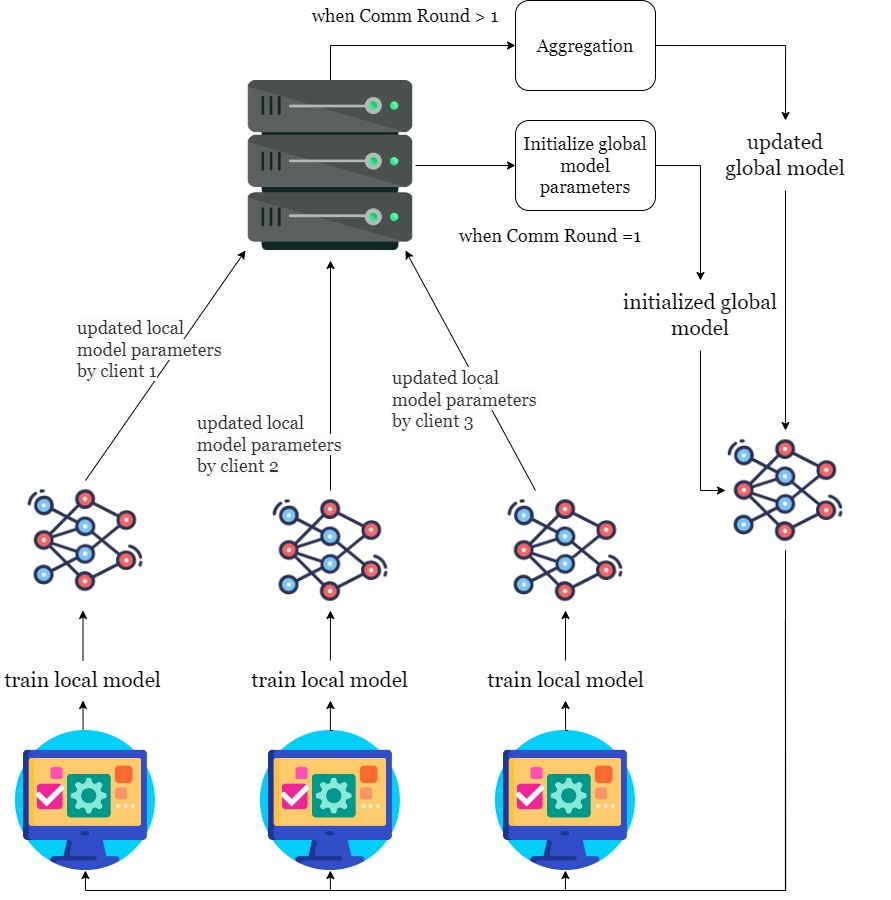
\includegraphics[width=100mm,height=92mm]{figures/federatedround.jpg}
\caption{Flowchart of federated learning}
\label{Flowchart of federated learning}
\end{figure}

\section{Federated Learning training algorithm}
\subsection{FedSGD (Federated Stochastic Gradient Descent)}
Stochastic Gradient Descent (SGD) can be applied to as a base to the Federated Learning training algorithm. A single batch gradient calculation is done on each round of communication. Although this approach is computationally efficient, it requires a large number of training rounds in order to produce good models. To apply this approach in the federated optimization problem, C-fraction of clients are selected on each round and the gradient of the loss is computed over all the data of the clients. Thus C is being used to control the global batch size, which when set to C=1, corresponds to full-batch (non-stochastic) gradient descent. This baseline algorithm is termed as FederatedSGD (or FedSGD).
\newline
The terms associated with the FedSGD computation are as follows: \newline
$ w_t $ = Model weights in communication round \#t \newline
$ w_t^k $ = Model weights in communication round \#t on client k \newline
C = Fraction of clients performing computations in each round \newline
E = Number of training passes each client makes over its local dataset on each round \newline
B = The local minibatch size used for the client updates \newline
$ \eta $ = The learning rate \newline
$ \Phi_k $ = Set of data points on client k \newline
$ \eta_k $ = Number of data points on client k \newline
$ f_i $ = Loss l($ x_i, y_i, z_i $) i.e., loss on example ($ x_i, y_i$) with model parameters w 

\subsection{FedAvg (Federated Averaging)}
One approach of FedSGD is that, the client computes the gradient, updates the model and sends it to the server. Now, if the model is updated multiple times before being sent to the server for aggregation, then the method is called FederatedAVG (or FedAVG).
% This helps to add more computation to each client, as the local update is iterated multiple times before the averaging is done. \newline
Here, the computation is kept in following parameters:\newline
C = Fraction of clients participating in that round\newline
E = No. of training passes each client makes over its local dataset each round\newline 
B = Local minibatch size used for client updates \newline
K = number of clients indexed by k ; \newline
The pseudo code for FedAVG algorithm is given below: 

% \begin{algorithm}
% \caption{Euclid’s algorithm}\label{euclid}
% \begin{algorithmic}[1]
% \Procedure{Euclid}{$a,b$}\Comment{The g.c.d. of a and b}
% \State $r\gets a\bmod b$
% \While{$r\not=0$}\Comment{We have the answer if r is 0}
% \State $a\gets b$
% \State $b\gets r$
% \State $r\gets a\bmod b$
% \EndWhile\label{euclidendwhile}
% \State \textbf{return} $b$\Comment{The gcd is b}
% \EndProcedure
% \end{algorithmic}
% \end{algorithm}

\begin{algorithm}
  \caption{Federated Learning Algorithm}
  
  \begin{algorithmic}
    \STATE \textbf{Server executes: \\}
    \STATE initialize $w_0$
    \STATE for each round $t=1,2, \ldots$ do \\
    \STATE $\quad  m \leftarrow \max (C \cdot K, 1)$ \\
    \STATE $\quad$ $S_t \leftarrow random \ set \ of \ $m$ \ clients $  \\
    \STATE $\quad$ for each client $k \in S_t$ in parallel do \\
    \STATE $\quad\quad\quad w_{t+1}^k \leftarrow$ ClientUpdate $\left(k, w_t\right)$ \\
    \STATE $\quad$ $w_{t+1} \leftarrow \sum_{k=1}^K \frac{n_k}{n} w_{t+1}^k$ \newline
    
    \STATE \textbf{ClientUpdate $(k, w): / /$} Run on client $k$ \\
    \STATE $\quad$ $\mathcal{B} \leftarrow\left(\right.$ split $\mathcal{P}_k$ into batches of size $\left.B\right)$ \\
    \STATE $\quad$ for each local epoch $i$ from 1 to $E$ do \\
    \STATE $\quad\quad$ for batch $b \in \mathcal{B}$ do \\
    \STATE $\quad\quad\quad\quad w \leftarrow w-\eta \nabla \ell(w ; b)$ \\
    \STATE $\quad$ return $w$ to server

  \end{algorithmic}
\end{algorithm}




		%--------------------------------
		
		%--------------------------------
		% Chapter 4: Result and analysis
		\chapter{METHODOLOGY}\label{METHODOLOGY}

This chapter discusses about the methodology that has been used to carry out the thesis work. The research is carried out using two approaches: Classical Machine Learning approach and Federated Learning approach.

\section{Identification of Research Gaps} 
Defining the system's goals and reading certain literature reviews are the first steps of the applied research methodology. The primary goals of the thesis are presented and the dataset of pap smear test cervical cell images is acquired. Then two approaches were followed for classification of those images.  

\section{Classical ML approach}
In this first approach, fifteen different Machine Learning models have been applied to train the model to determine which would provide an overall increased accuracy. Subsequently, the models are compared with respect to the accuracy, precision, recall and f1-score of the training set and the accuracy, precision and recall of the test set.

\section{Federated Learning Approach}
In the second approach, various CNN models were developed and integrated with FL architecture. Hyperparameter tuning was done to figure out the best possible architecture. After evaluating the models, the best model was deployed through streamlit and a user interface was designed in order to apply the proposed system in a real-world environment. 

\begin{figure}[H]
\centering
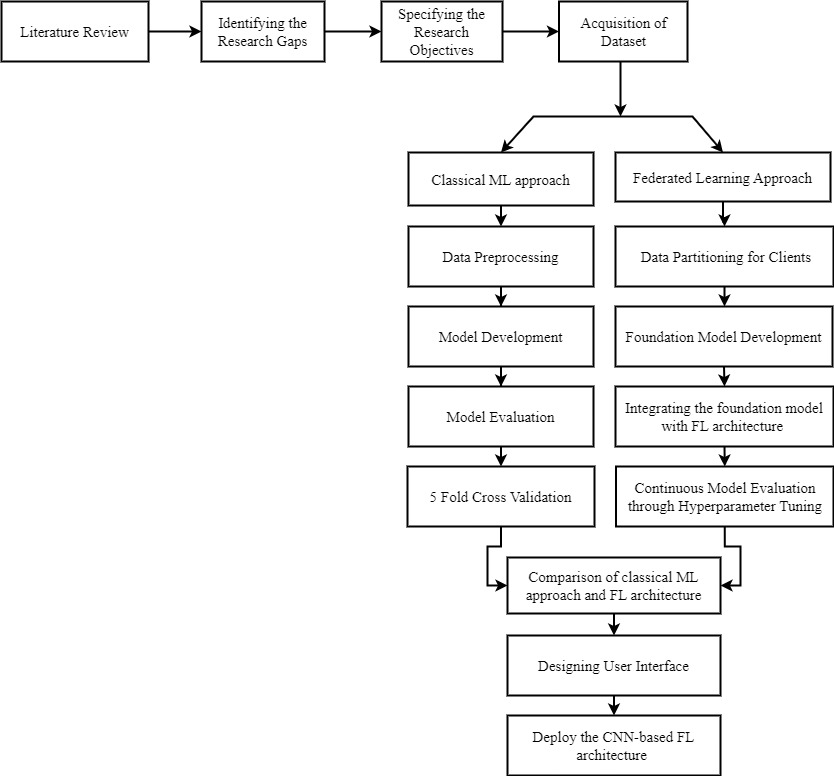
\includegraphics[width=148mm,height=140mm]{figures/meth.jpg}
\caption{Overview of Methodology}
\label{DLAccuracy}
\end{figure}

An overview of methodology is shown in Fig 4.1. By following this methodology, a conclusion was reached that FL performs significantly better than classical ML models.


\endinput


		%--------------------------------
		\include{chapters/chapter5_result}
		\chapter{CONCLUSION}\label{conclusion}


This chapter puts forth the summarization of the overall thesis by using four subsections to demonstrate the thesis’s overview, contribution, limitations, and scope for future work

\section{Thesis Overview}
% \section{Thesis Outcome}
The main objective of this thesis is to introduce a system which will be able to classify cervical cancer cells by ensuring privacy. A detailed literature study was conducted to get better knowledge for the development of the system. The exploration aided in knowing about the application of federated learning in classification through data collection. Since very less work has been done, this study tries to incorporate Federated learning in cervical cancer classification. This work helps to avoid data sharing which was of a signifcant challenge in the related works of the past. The work introduces a personalized convolutional neural network for the purpose of classification, which was not introduced in the works before. 

The outcome of the thesis is the development of a system that makes use of a novel deep learning architecture, which makes use of the privacy ensured by Federated Learning, for the classification of any input cervical cancer cell.

\section{Thesis Contribution}
The main contribution of this thesis is the development of an interactive web application for classification of cervical cancer cells. The Deep Learning model, incorporated with the FL architecture that can operate well even with small-sized datasets. Thus the system does not require a heavy setup of devices. The system has a centralized global model and initially untrained local models, allocated for each client. The clients train the local models with their dataset, and only the updated local models get aggregated with the global model, thus ensuring privacy as their data is never collected centrally. Thus, through this system, clients from any part of the world can help to improve the accuracy of the model, without having to share their data. This helps to gain an overall enriched model as various types of data get combined for the development of the global model.
In some recent works classification of cancer cells incorporating federated can be found, but the approaches have not introduced the development of a customized Convolutional Neural Network. A novel deep learning model, integrated with Federated Learning can result in an improved classification system even with the dearth of a large amount of data.

\section{Thesis Limitations and Future Work}
A few limitations of the thesis are: 
\begin{enumerate}
    \item
    The method considers the development of a Deep Learning model, which is very time consuming owing to its high computational capacity.
    \item
    The proposed system incorporated data from only three hospitals. The effectiveness of the system may be improvised by the introduction of more hospitals in the future.
    \item
    Although crucial for accurate results, acquiring sufficient quantity of data for training purposes poses a significant limitation.
    
\end{enumerate}
The future work will focus on introducing differential privacy which would help to give as accurate results as possible while maintaining privacy by enabling the quantification of the extent of privacy of a database. By deploying in the real world, the system can be upgraded through continuous user feedback. And finally, different algorithms can be tested in the future to find out which may result in better accuracy.



\endinput
		%--------------------------------
		% Chapter 5: Conclusion and future work
		
		
	}
	%--------------------------------
	
	%--------------------------------
	%List of Publications
	%% !TEX root = ../thesis.tex
\cleardoublepage
\phantomsection
\addcontentsline{toc}{chapter}{LIST OF PUBLICATIONS}
\chapter*{\large LIST OF PUBLICATIONS}
%\begin{listofpublications}
\label{listofpublications}



%ADD MORE ITEMS OR DELETE ITEMS IF YOU REQUIRE
\noindent {\large \bf Journal Papers:}
\begin{enumerate}
%%
\item[(i)] 
\textbf{Authors-Lastname, F. N.} and Others-Lastname, F. N., 
``Article title,''
\emph{Name of the Journal}, 
Publisher, 2019.

\item[(ii)] 
\textbf{Authors-Lastname, F. N.} and Others-Lastname, F. N., 
``Journal-Article title,''
\emph{Name of the Journal}, 
Publisher, 2019. (under review)

\end{enumerate}
%
%
\noindent {\large \bf Conference Papers:}
\begin{enumerate}

\item[(iii)] 
\textbf{Authors-Lastname, F. N.} and Others-Lastname, F. N., 
``Conference paper title" 
\textit{Proceedings title}, 
City of the conference,
Country,
Publisher, 
year,
pp. xx-xx. 

\item[(iv)]
\textbf{Authors-Lastname, F. N.} and Others-Lastname, F. N., 
``Conference paper title" 
\textit{Proceedings title}, 
City of the conference,
Country,
Publisher, 
year,
pp. xx-xx. 


\item[(v)]
\textbf{Authors-Lastname, F. N.} and Others-Lastname, F. N., 
``Conference paper title" 
\textit{Proceedings title}, 
City of the conference,
Country,
Publisher, 
year,
pp. xx-xx. 


\end{enumerate}


%\item[(v)]
%%\textbf{M.~A. Wahed} and H.~Nyeem, ``Modeling and analysis of interpolation based adaptive reversible data
%%  hiding,'' in \emph{Proc. of EICT 2017}, IEEE, 2017.
%%
%%\item[(vi)]
%%\textbf{M.~A. Wahed} and H.~Nyeem, ``Efficient data embedding for interpolation based reversible data
%%  hiding scheme,'' in \emph{Proc. of ICEEE 2017}, IEEE, 2017.
%%
%%\item[(vii)]
%%\textbf{M.~A. Wahed} and H.~Nyeem, ``Efficient LSB substitution for interpolation based reversible data
%%  hiding scheme,'' in \emph{Proc. of ICCIT 2017}, IEEE, 2017  (\textbf{best paper award}).

%%\end{listofpublications}
%

	%\addcontentsline{toc}{chapter}{LIST OF PUBLICATIONS}
	%\listofpublications 
	%--------------------------------
	
	%--------------------------------
	% References
% 	{\small
% 		\bibliographystyle{IEEETran}
% 		\cleardoublepage
% 		\phantomsection
% 		\addcontentsline{toc}{chapter}{REFERENCES}
% 		\bibliography{MyReferences.bib}
% 	}
    
    % \bibliographystyle{agsm}
    \bibliographystyle{apacite}
    \bibliography{ref}
    


	%--------------------------------
	
	%--------------------------------
	% Appendix
	\appendix
	\renewcommand\appendixname{APPENDIX}
	% 
\begin{appendices}
\raggedbottom

\chapter{CODES}
\label{matlab}
%\setlength{\leftmargin}{2in}%
\section{Data Preprocessing}
Data was preprocessed by using following code.
\lstinputlisting{codes/text_preprocessing.py}

%%%%%%%%%%%%%%%%%%%%%%%%%%%%%%%%%%%%%%%%%%%%%%%%%%%%%%%%
\vspace{2.5ex}
\section{Neural Network Models}
Three neural network models were developed using following codes.
\subsection{Developing LSTM model}
\lstinputlisting{codes/lstm.py}
\subsection{Developing BiLSTM model}
\lstinputlisting{codes/bilstm.py}

\vspace{2.5ex}


\end{appendices}
	%\titlelabel{\thetitle\ - }
	%--------------------------------
	%\lstinputlisting{../bfsPVOfullRun.
	
	% \afterpage{\blankpage}

\end{document}